\begin{abstract}

Smart building energy management requires better load forecast models and better control strategies, within each cluster there are considerable research advances over the past few years. Improving the economic performances in real-world practice asks for seamlessly integration of the two parts, however, comprehensive uncertainty quantification is very limited.  
In this research, we focus on understanding how forecast errors on building electricity load impact control performances under model predictive control (MPC) strategies, i.e., quantifying the value of information (VoI) for building energy management. We implement a collection of both cutting-edge and common-practice learning algorithms for building load forecast, and formulate a MPC pipeline that uses the forecast information for building energy control. With extensive simulations based on real scenarios, our findings demonstrate that: first, MPC strategies have heterogeneous sensitivities on forecast errors under different energy pricing schemes. Specifically, they are robust when the electricity bill does not include demand charges, but become extremely sensitive to even tiny errors when demand charge is introduced. Second, we uncover that forecasting errors have asymmetric impact on control performances that underestimations of load consequence a more detrimental effect on MPC performance compared to overestimations. 
Our study implies that researchers should consider the learning and optimization tasks as a whole: on the one hand, we should define better error metrics which characterizes the specific downstream control challenges when fitting load forecast models. On the other hand, when designing control strategies, robustness under forecast errors should be carefully considered.


% Microgrid optimization is crucial for economic efficiency, sustainability, and grid stability, with Model Predictive Control (MPC) offering a promising approach. Microgrid utility bills typically comprise both electricity usage charges and demand charges, with the latter being linked to peak power consumption during billing cycles. As a predictive control strategy, to implement MPC requires accurate load forecasting during the control horizon. In this research, we employ representative machine learning algorithms and heuristic models for load forecasting, with a specific focus on understanding how forecast uncertainties would impact control performance, particularly in the presence of demand charges. Our findings demonstrate that MPC, when operating without including demand charges, exhibits robustness against forecast uncertainties, yielding nearly optimal performance even when forecast errors reach 10\% Mean Absolute Percentage Error (MAPE). However, when demand charges are introduced, even minor prediction errors as low as 1\% MAPE lead to significantly worse control outcomes. We further uncover that this disparity arises from the asymmetric impact of forecasting errors, where underestimations of load have a more detrimental effect on MPC performance compared to overestimations. Moreover, we identify the limitations associated with employing singular aggregate metrics such as MAPE as indicators for MPC forecasts. We emphasize the importance of considering residual patterns and temporal correlations among consecutive steps to obtain a comprehensive evaluation of forecasting accuracy. Consequently, this study advocates for a thorough examination of forecasting features to establish a clear objective for upstream forecasting tasks, aiming at enhancing the performance and effectiveness of MPC in microgrid energy management.

\end{abstract}

\keywords{
 Prediction uncertainty \and Model predictive control \and Building load forecast \and Smart grid operation
}

\newcommand{\R}{\mathbb{R}}
\newcommand{\N}{\mathbb{N}}
\newcommand{\Z}{\mathbb{Z}}
\newcommand{\Q}{\mathbb{Q}}

\newcommand{\prob}[1]{\mathbb{P}\left\{#1\right\}}
\newcommand{\ept}[1]{\mathbb{E}\left\{#1\right\}}
\newcommand{\Var}[1]{\text{Var}\left\{#1\right\}}
\newcommand{\ind}[1]{\mathbf{1}\left\{#1\right\}}

\newcommand{\relu}[1]{\left[ #1 \right]^{+}}
\newcommand{\reluN}[1]{\left[ #1 \right]^{-}}
\newcommand{\tset}{\mathcal{T}}

\newcommand{\dt}{\Delta_t}
\newcommand{\dk}{\Delta_k}
\newcommand{\tou}{\gamma}
\newcommand{\dc}{\overline{\gamma}}

\newcommand{\pgrid}{p^{\text{G}}}
\newcommand{\pgridU}{\overline{P}^\text{G}}
\newcommand{\pgridL}{\underline{P}^\text{G}}
\newcommand{\pDC}{p^\text{DC}}
\newcommand{\pDCt}{p^\text{DC}_{t}}

\newcommand{\pbatt}{p^\text{B}}
\newcommand{\ebatt}{b}
\newcommand{\effbatt}{\eta}
\newcommand{\pbattL}{\underline{P}^\text{B}}
\newcommand{\pbattU}{\overline{P}^\text{B}}
\newcommand{\ebattL}{\underline{B}}
\newcommand{\ebattU}{\overline{B}}

\newcommand{\pev}{p^\text{EV}}
\newcommand{\eev}{e}
\newcommand{\effev}{\xi}
\newcommand{\pevL}{\underline{P}^\text{EV}}
\newcommand{\pevU}{\overline{P}^\text{EV}}
\newcommand{\eevL}{\underline{E}}
\newcommand{\eevU}{\overline{E}}
\newcommand{\evind}{\mathbb{I}}
\newcommand{\ta}{\tau^{\text{a}}}
\newcommand{\td}{\tau^{\text{d}}}
\newcommand{\edem}{E^\text{dem}}
\newcommand{\einit}{E^\text{init}}
\newcommand{\etarg}{E^\text{targ}}
\newcommand{\Iset}{\mathcal{I}}

\newcommand{\indtilde}{\widetilde{\mathbb{I}}}
\newcommand{\tdtilde}{\widetilde{\tau}^{\text{d}}}

\newcommand{\pevUest}{\widehat{\underline{P}}^\text{EV}}
\newcommand{\pevLest}{\widehat{\overline{P}}^\text{EV}}
\newcommand{\eevUest}{\widehat{\underline{E}}}
\newcommand{\eevLest}{\widehat{\overline{E}}}
\newcommand{\indest}{\widehat{\mathbb{I}}}
\newcommand{\taest}{\widehat{\tau}^{\text{a}}}
\newcommand{\tdest}{\widehat{\tau}^{\text{d}}}
\newcommand{\edemest}{\widehat{E}^\text{dem}}
\newcommand{\einitest}{\widehat{E}^\text{init}}
\newcommand{\etargest}{\widehat{E}^\text{targ}}
\newcommand{\Iest}{\widehat{\mathcal{I}}}

\newcommand{\pbld}{P^\text{D}}
\newcommand{\ppv}{P^\text{PV}}
\newcommand{\bldest}{\widehat{P}^\text{D}}
\newcommand{\pvest}{\widehat{P}^\text{PV}}

\newcommand{\tToK}{t_{[K]}}
\newcommand{\pgridSch}{\widetilde{p}^{\text{G}}}
\newcommand{\pbattSch}{\widetilde{p}^{\text{B}}}
\newcommand{\pevSch}{\widetilde{p}^{\text{EV}}}
\newcommand{\prevmax}{P^{\max}}
\newcommand{\prevmaxNecc}{\widetilde{P}^{\max}}

\newcommand{\bldavg}{\overline{P}^{\text{D}}}

\newcommand{\avepbld}{\mu_\text{bld}}
\newcommand{\rpv}{\phi_\text{pv}}
\newcommand{\rev}{\varphi_\text{ev}}
\newcommand{\rbat}{k_\text{bat}}

\newcommand{\wodc}{\mathbf{{DC}^{0}}}
\newcommand{\wdc}{\mathbf{{DC}^{+}}}
\newcommand{\MPCe}{\textbf{MPC-${\epsilon }$} }

\newcommand{\kexe}{K_{exe}}
\newcommand{\kgt}{K_{GT}}


% \color{blue}
% \section*{Notes for co-authors}
% \begin{enumerate}
%     \item You can find the structure of this manuscript in \texttt{main.tex}. Each section is written in a separate file under the folder \texttt{content\textbackslash}. I create many shortcuts for variable names, which you can find in \texttt{0-newcommands.tex}.
%     \item I highlight what is missing / I am quite unsure in \textcolor{red}{red}.
%     \item For quicker rendering, I use figures of low resolution now, and I will replace them with high quality version before submission.
%     \item Please check that \emph{track changes} is on for you (click the 'Review' button on the upper line).
%     \item Do we need to emphasize more on the relevance of our paper with the session theme  - I am afraid it is not quite strong currently.
% \end{enumerate}
% \color{black}

\section{Introduction} \label{sec:intro}
%\lunlong{Introduction not drafted yet}

\subsection{Background}
Smart microgrids that incorporate distributed energy resources (DERs) play a crucial role in the pursuit of achieving carbon neutrality by integrating renewable energy generation \cite{li2023modeling}. However, this integration introduces significant challenges to the design, planning, and operation of the energy system. One prominent challenge is the growing temporal mismatch between renewable energy generation and peak electricity demand, known as the "Duck Curve" \cite{DuckC_ES}. The Duck Curve exhibits two distinct features. Firstly, there is a substantial decline in net demand (total electricity demand minus renewable generation) during midday when solar energy generation is high \cite{wang2023site}, represented by the curve's ``belly." This excess electricity production often leads to renewable curtailment. Secondly, there is a rapid increase in net demand, resembling the curve's ``head." Meeting this sudden demand requires grid operators to rely on large-scale fossil fuel generators as backup, which is costly and environmentally detrimental. This temporal imbalance strains the grid and poses challenges to the operation of smart grids \cite{widjaja2023general}.

Addressing the challenges posed by the duck curve involves implementing energy storage solutions such as electrical energy storage (e.g., batteries) or thermal energy storage (e.g., chilled water tanks or ice storage). However, integrating renewable generation and energy storage increases system complexity, necessitating dedicated algorithms for system operation. Advanced control algorithms like Model Predictive Control (MPC) \cite{kim2022site} and Reinforcement Learning (RL) \cite{touzani2021controlling} have been employed to optimize the coordination between building HVAC systems and energy storage, demonstrating superior performance compared to traditional rule-based control (RBC) strategies.

To optimize the design and operation of multiple heterogeneous but interconnected energy subsystems in an effective and reliable way is challenging \cite{Energy_model_complex}, as this optimization is information-intensive. The predicted information about the building load, renewable generation is needed in this predictive control paradigm. How to obtain and process the extensive information to make reasonable predictions in an online manner is crucial for making informed decisions in microgrids \cite{Intensive_data_grid}.

\subsection{Existing Works}

\subsubsection{Smart grid operation }

Smart grid operation involves the coordination of multiple energy systems, such as energy storage charging/discharging, electric vehicle charging, and space pre-cooling/pre-heating, in an efficient and reliable way \cite{dong2023modeling}. Within this domain, three main control paradigms are commonly employed: rule-based control (RBC), model-predictive control (MPC), and reinforcement learning (RL). RBC relies on a predefined set of rules to govern the operation of the smart grid. Examples of RBC strategies include maximizing self-consumption (MSC) and Time-of-Use (TOU) approaches discussed in \cite{zou2022comparative}. Currently, RBC strategies dominate the industry due to their simplicity and interpretability. However, a drawback of RBC is that the predetermined rules often fail to lead to optimal control actions.

MPC and RL are two emerging advanced control strategies in the field of smart grid management research and applications. MPC formulates an optimization control problem based on a physical model of the dynamic system and repeatedly re-optimizes as new system states are observed \cite{hu2021model}. In contrast, RL aims to learn a control strategy directly from reward maximization using a Markov decision process (MDP), without explicit knowledge of the system dynamics \cite{wang2020reinforcement}. Although both MPC and RL are optimization-based control strategies, they differ in their approach to decision-making. MPC relies on a model of the system dynamics to make informed decisions, while RL takes a model-free approach by relying on data. Compared to RL, MPC is considered more data-efficient and interpretable for energy system management \cite{wang2023comparison}. As a result, it has been extensively explored in the literature for various applications such as electric vehicle charging coordination \cite{shi2018model}, thermal storage operations \cite{tang2019model}, and hydrogen energy systems \cite{RenewMG_reduc_DC}. MPC has also been demonstrated in field studies, as exemplified by \cite{MPC_insitu}.

Within the microgrid context, economic Model Predictive Control (MPC) aims to optimize various control objectives, which may include utility costs, carbon emissions, system stability, and occupant satisfaction \cite{MEMS_LR}. Utility costs typically comprise two primary components: energy charges and demand charges. Energy charges are determined based on the amount of electricity consumed, and the pricing scheme may consider factors such as time of day, season, and overall consumption levels \cite{fernandez2023demand}. On the other hand, demand charges are calculated based on the maximum power demand observed by the consumer during a billing cycle, and for certain commercial electricity consumers, they can account for more than half of the total electric bill. Houben et al. \cite{uncertainty_dc} highlighted that the inability to accurately predict peak demand may lead to insufficient energy stored in the battery energy storage system (BESS) to avoid a new peak demand, resulting in additional costs.

\subsubsection{Building load prediction}

The initial step towards predictive control involves making predictions regarding building load and renewable generation. Building load prediction is an area of active research due to its broad applications in optimizing HVAC control \cite{kusiak2010cooling}, operating thermal energy storage systems \cite{luo2017data}, planning energy distribution systems\cite{pedersen2008load}, and managing smart grids \cite{xue2014interactive}. 

Approaches for forecasting building thermal load can be broadly classified into three categories: white-box physics-based models, gray-box reduced-order models, and black-box data-driven models\cite{wang2020building}. White-box models utilize detailed heat and mass transfer equations to predict building loads. Commercial software tools like EnergyPlus, Dest, and TRNSYS are available for setting up white-box models \cite{li2014review}. Black-box models, on the other hand, rely solely on historical data to predict building thermal load. Gray-box models simplify the building's thermal dynamics by using reduced-order Resistance and Capacity (RC) models, and then estimate parameter values using historical data. For smart grid operations, black-box data-driven models are widely preferred for two main reasons. Firstly, advancements in machine learning algorithms and the increased availability of historical data have made black-box models more accurate \cite{liu2023timetabling}. Secondly, developing physics-based models requires extensive input data, including thermal properties of the building envelope, occupancy and equipment schedules, which can be time-consuming, if not totally impossible, to gather. Some widely used black-box load prediction models will be introduced in greater details in Section. \ref{section:Building load forecasts}.

However, due to limited access to high-quality training data, potential changes in energy usage patterns, and system behaviors, uncertainties may arise in both demand and generation predictions \cite{tian2022daily}. Additionally, limited research directly addresses load prediction accuracy in specific downstream tasks. Studies have shown that under Model Predictive Control (MPC) or its surrogate neural networks (NN), the requirement for prediction accuracy appears to be moderate \cite{sun2016nonlinear, wu2022learning}. However, these evaluations do not consider demand charges. Gust et al. suggest that such conclusions may not hold when demand charges are taken into account \cite{gust2021strategies}. Stochastic programming is a general solution for addressing these challenges, but it often leads to a substantial increase in computational complexity.

\subsection{Scope and objectives}

Our literature review revealed a significant gap in the analysis of load forecast information's value in microgrid energy management, particularly in relation to the presence or absence of demand charges. This gap represents a notable disparity between two prominent clusters of research in the field. It is important to note that this concern has garnered attention from researchers within the broader context of \emph{integrated learning \& optimization} (ILO). For instance, Silwal et al. \cite{elmachtoub2022smart} propose a loss function, along with its convex surrogate, SPO+, which explicitly incorporates the optimization problem structure into the prediction loss. These pioneering works offer valuable intellectual insights; however, their applicability is unfortunately limited to a specific class of problems.

In this work, we aim at investigating the impact of building load forecasts on MPC of the microgrid, and examining the influences of demand charge in microgrid management. Our specific objectives are as follows:
\begin{enumerate}
    \item Perform a systematic review and residual analysis on cutting-edge and well-adopted load forecast models.
    \item Quantify the VoI of building energy management tasks through a realistic MPC pipeline under various scenarios. Specifically, we compare the cases with and without demand charge.
    \item Conduct parametric experiments to examine the correlations between the forecast residual patterns and downstream control performances. Specifically, we unveil the asymmetric effect of forecast errors.
    %\item Found that the impact of prediction errors are asymmetric: underestimating load leads to more sub-optimal control outcome than overestimating the load with the existence of demand charge.
    %\item Reveal that conventional lump metrics widely used in the forecasting tasks are not suitable for microgrid energy management under MPC, when demand charge is considered.
\end{enumerate}

The rest of the manuscript is organized as follows: Sec. \ref{sec:method} details the workflow of this study, including forecasting approaches, control model for microgrid energy management and configurations for the simulations. Then in Sec. \ref{sec:results}, we present the results of the simulations. In Sec. \ref{sec:discussion}, we discuss and extend the results, before we conclude in Sec. \ref{sec:conclusion}.
%Sec.\,\ref{sec:model} details the optimal control model for microgrid energy management, followed by Sec.\,\ref{sec:VoI} that discusses the value of building load information and the role of peak power tracking. We perform comprehensive numerical studies to demonstrate our findings and validate our proposed approach in Sec.\,\ref{sec:results}. The manuscript is concluded in Sec.\,\ref{sec:conclusion}.





% \section{Method} \label{sec:model}
% In this section, we articulate an optimal energy management model under general microgrid settings.

\subsection{Nomenclature}
% \lunlong{Maybe the explanation of OPEX, TOU should be placed here?}
In this paper, we denote the set of real numbers by $\R$ and the set of integers by $\Z$. We use functions $\ind{\cdot}$, $[\cdot]^{+}$, $[\cdot]^{-}$, $\lfloor \cdot \rfloor$ in their conventional meanings, i.e., $\ind{x}=1$ if $x$ is true otherwise $\ind{x}=0$, $[x]^{+} \coloneqq \max\{0,x\}$, $[x]^{-} \coloneqq \min\{0,x\}$.\footnote{
For consistency, we adopt the convention that using lowercase letters (e.g., $x$) for (decision) variables, uppercase letters (e.g., $X$) and Greek letters (e.g., $\alpha$) for parameters, and calligraphic uppercase letters (e.g., $\mathcal{X}$) for sets.}

\subsection{System Configuration}
Without loss of generality, we consider an external-grid-connected microgrid with distributed solar panel (PV) generation, and battery energy storage. The loads of the microgrid includes building energy consumption, as well as EV charging demands. Specifically:

\begin{itemize}
    \item At time $t$, building load $\pbld_t$ and PV generation $\ppv_t$ are assumed to be uncontrollable.
    \item The microgrid can import electricity power from, or export to the external grid, which is $\pgrid_t$ at time $t$ (negative for export), at time-of-use (TOU) tariff $\tou^+_t$ (purchase) or $\tou^-_t$ (sell).
    \item A battery with capacity $B$ and maximum discharging (charging) power $\pbattU$ ($\pbattL$). At time $t$, its discharging power is $\pbatt_t$, for which negative value indicates charging.
    \item EV charging demands are considered to be dispatchable. For EV $i$, which is plugged-in during $\ta_i$ to $\td_i$ with initial charge $\einit_i$, it should be charged to $\etarg_i$ by its departure. At time $t$, the charging power of EV $i$ is $\pev_{i,t}$, for which negative value indicates discharging. %\scott{At this point, the controllable EV charging seems like an unnecessary complication given the key research question and contribution.}
    \item A \emph{demand charge} term is included as part of the utility bill, which has a constant marginal rate $\dc$ (per kW) applied to the maximum consumed power $\pDC$ within the billing cycle.% And the latest maximum consumed power at time $t$ is $\pDCt$.
\end{itemize}

\subsection{Optimal Energy Management}
\begin{subequations}

The goal of the optimization is to minimize the electricity bills over horizon $\tset = \{0,1,...,T\}$, i.e.,:
\begin{equation}\label{eq:opt_obj}
    \sum_{t=0}^{T-1} \left\{ 
           \tou_t^+ \relu{\pgrid_t} - \tou_t^- \reluN{\pgrid_t} \right\} \dt
           + \dc \, \pDC
\end{equation}
which is the consumption-based cost plus the demand charge. $\pDC = \max_t~ \{\pgrid_t\}$, which is the maximum grid import power within a billing cycle.\footnote{For simplicity, we consider $\tset$ contains one billing cycle, which is typically one month.} We can reformulate the maximum equality as:
\begin{equation}\label{eq:constr_dc}
    \pDC \ge \pgrid_t, ~~~~ \forall ~t
\end{equation}


Supply-demand balance should be observed at every time step:
\begin{equation}
    \pgrid_t + \pbatt_t + \ppv_t = \pbld_t + \sum_{i=1}^I \pev_{i,t},
                ~~~~ \forall ~ t
\end{equation}

Power imported from or exported to external grid is limited:
\begin{equation}
   \pgridL \le \pgrid_t \le \pgridU, ~~~~\forall ~t
\end{equation}
If $\pgridL = \pgridU = 0$, the microgrid is isolated. In general, such limits are determined by the transformer capacity, per certain microgrid codes.

For the battery, the following constraints (dynamics) need to be satisfied\footnote{We consider an ideal battery model here for simplicity. We will plug in more complicated models, e.g., considering battery degradation, in our future work for sensitivity analysis.}:
\begin{align}
   & \ebatt_{t+1} = \ebatt_t  + \left(\effbatt^- \reluN{\pbatt_t} - \frac{1}{\effbatt^+} \relu{\pbatt_t}\right) \dt,
                ~ \forall ~ t \\
   & \pbattL \le \pbatt_t \le \pbattU,~~~~ \forall ~ t\\
   &  \ebattL \le \ebatt_t \le \ebattU,~~~~ \forall ~ t\\
   & b_0 = B_0 , ~~ b_T \ge B_T
\end{align}
where $\effbatt^+$ ($\effbatt^-$) is the discharging (charging) efficiency.

For each EV $i$, its charging schedule should follow the following constraints:
\begin{align}
    & \eev_{i,t+1} = \eev_{i,t} + \left(\effev^+ \relu{\pev_{i,t}} - \frac{1}{\effev^-} \reluN{\pev_{i,t}}\right) \dt,
                ~~\forall ~ t\\
   & \pevL_i\, \evind_{i,t} \le \pev_{i,t} \le \pevU_i\, \evind_{i,t}, 
        ~~~~\forall ~ t\\
   &  \eevL_i \le \eev_{i,t} \le \eevU_i,
        ~~~~\forall ~ t\\
   & e_{i,\ta_i} = \einit_i, ~~ e_{i,\td_i} \ge \etarg_i \label{eq:constr_e_init_targ}
\end{align}
where $\evind_{i,t} = \ind{\ta_i \le t < \td_i}$ indicates whether EV $i$ is in the station at time $t$, and $\xi^+$ ($\xi^-$) is the charging (discharging) efficiency. The formulation is compatible with different charging modes. For example, bidirectional charging, a.k.a., vehicle-to-grid (V2G) can be allowed by setting $\pevL_i = - \pevU_i$, or prohibited with $\pevL_i=0$. If the charging process is uncontrollable, we can pre-calculate $\pevL_{i,t} = \pevU_{i,t}$ thus $\pev_{i,t}$ is pre-determined.
\end{subequations}

To conclude, a general formulation of optimal energy management is:
\begin{subequations}\label{eq:opt1}
    \begin{align}
        \min~~ & \text{obj. \eqref{eq:opt_obj}}\\
        \text{s.t.~~~~} & \text{constr. \eqref{eq:constr_dc}-\eqref{eq:constr_e_init_targ}}
    \end{align}
\end{subequations}
With some trivial reformulations, the program \eqref{eq:opt1} is a linear programming (LP).\footnote{Some assumptions, e.g., $\tou^+_t \ge \tou^-_t$ are required, which are also trivial.}

\section{Method} \label{sec:method}


% \yi{consider re-organize this section: detail on our meeting ...}

% \subsection{Research outline}
    %\subsubsection{Data preparation}
In this section, we present the work stream involved in MPC of microgrid energy management. The application of MPC consists of two main stages in this study: forecasting and optimization. In order to be coherent, we first introduce the optimization task and related concepts in Sec. \ref{section:MEM}, then detail the load forecasting in Sec. \ref{section:Building load forecasts}. 
In the initial stage, predictions for the loads are made based on historical data and other relevant information. Machine learning approaches and heuristic methods are used for forecasting in this study. Several lump metrics are included to evaluate the forecasting accuracy.
Then an optimization problem is formulated for MPC, which takes various control variables into account and is subjected to specific constraints. Its objective is to find the control actions that minimize the performance criterion (i.e., utility cost in this study). In order compare the control performance of MPC with different forecasts, we consider rule base control (RBC) as a benchmark. RBC is a controlling technique that does not rely on forecasts, based on which the concept value of information is proposed as a metric. 
At the end, two experimenting scenarios considering different billing schemes and corresponding configurations are introduced in Sec. \ref{section:configurations}.

%============================================================================================================
\subsection{Microgrid energy management} %-------------------------------------------------------------------
\label{section:MEM}
\subsubsection{System Configuration}

In this paper, we denote the set of real numbers by $\R$ and the set of integers by $\Z$. We use functions $\ind{\cdot}$, $[\cdot]^{+}$, $[\cdot]^{-}$, $\lfloor \cdot \rfloor$ in their conventional meanings, i.e., $\ind{x}=1$ if $x$ is true otherwise $\ind{x}=0$, $[x]^{+} \coloneqq \max\{0,x\}$, $[x]^{-} \coloneqq \min\{0,x\}$.\footnote{
For consistency, we adopt the convention that using lowercase letters (e.g., $x$) for (decision) variables, uppercase letters (e.g., $X$) and Greek letters (e.g., $\alpha$) for parameters, and calligraphic uppercase letters (e.g., $\mathcal{X}$) for sets.}
    
We consider a typical external-grid-connected microgrid, which is distributed with solar panel (PV) generation and battery energy storage system (BESS). The loads of the microgrid is building energy consumption. Specifically:

\begin{itemize}
    \item At time $t$, building load $\pbld_t$ and PV generation $\ppv_t$ are assumed to be uncontrollable.
    \item The microgrid can import electricity power from, or export to the external grid, which is $\pgrid_t$ at time $t$ (negative for export), at time-of-use (TOU) tariff $\tou^+_t$ (purchase) or $\tou^-_t$ (sell).
    \item A battery with capacity $B$ and maximum discharging (charging) power $\pbattU$ ($\pbattL$). At time $t$, its discharging power is $\pbatt_t$, for which negative value indicates charging.
    \item A \emph{demand charge} term is included as part of the utility bill, which has a constant marginal rate $\dc$ (per kW) applied to the maximum consumed power $\pDC$ within the billing cycle.% And the latest maximum consumed power at time $t$ is $\pDCt$.
\end{itemize}

\subsubsection{Optimal Energy Management} %------------------------------------------------------------------

\begin{subequations}
The goal of the optimization is to minimize the electricity bills over horizon $\tset = \{0,1,...,T\}$, i.e.,:
\begin{equation}\label{eq:opt_obj}
    \sum_{t=0}^{T-1} \left\{ 
           \tou_t^+ \relu{\pgrid_t} - \tou_t^- \reluN{\pgrid_t} \right\} \dt
           + \dc \, \pDC
\end{equation}
which is the consumption-based cost plus the demand charge. $\pDC = \max_t~ \{\pgrid_t\}$, which is the maximum grid import power within a billing cycle.\footnote{For simplicity, we consider $\tset$ contains one billing cycle, which is typically one month.} We can reformulate the maximum equality as:
\begin{equation}\label{eq:constr_dc}
    \pDC \ge \pgrid_t, ~~~~ \forall ~t
\end{equation}

Supply-demand balance should be observed at every time step:
\begin{equation}
    \pgrid_t + \pbatt_t + \ppv_t = \pbld_t ,
                ~~~~ \forall ~ t
\end{equation}

Power imported from or exported to external grid is limited:
\begin{equation}
   \pgridL \le \pgrid_t \le \pgridU, ~~~~\forall ~t
\end{equation}
If $\pgridL = \pgridU = 0$, the microgrid is isolated. In general, such limits are determined by the transformer capacity, per certain microgrid codes.

For the battery, the following constraints (dynamics) need to be satisfied\footnote{We consider an ideal battery model here for simplicity. We will plug in more complicated models, e.g., considering battery degradation, in our future work for sensitivity analysis.}:
\begin{align}
   & \ebatt_{t+1} = \ebatt_t  + \left(\effbatt^- \reluN{\pbatt_t} - \frac{1}{\effbatt^+} \relu{\pbatt_t}\right) \dt,
                ~ \forall ~ t \\
   & \pbattL \le \pbatt_t \le \pbattU,~~~~ \forall ~ t\\
   &  \ebattL \le \ebatt_t \le \ebattU,~~~~ \forall ~ t\\ 
   & b_0 = B_0 , ~~ b_T \ge B_T \label{eq:constr_e_init_targ}
\end{align}
where $\effbatt^+$ ($\effbatt^-$) is the discharging (charging) efficiency.

\end{subequations}

To conclude, a general formulation of optimal energy management is:
\begin{subequations}\label{eq:opt1}
    \begin{align}
        \min~~ & \text{obj. \eqref{eq:opt_obj}}\\
        \text{s.t.~~~~} & \text{constr. \eqref{eq:constr_dc}-\eqref{eq:constr_e_init_targ}}
    \end{align}
\end{subequations}
With some trivial reformulations, the program \eqref{eq:opt1} is a linear programming (LP).\footnote{Some assumptions, e.g., $\tou^+_t \ge \tou^-_t$ are required, which are also trivial.}

\subsubsection{Model predictive control (MPC)} %------------------------------------------------------------------

Compactly, we write the constrained finite-time optimal control (CFTOC) problem as:
\begin{equation}
    \widetilde{u}_{t_{[K]}} = \arg\min J(u_{t_{[K]}} \mid x_t, w_{t_{[K]}}, \theta_{t_{[K]}})
\end{equation}
where $z_{t_{[K]}} = \{z_t, z_{t+1}, ..., z_{t+K}\}$, and $x, u, w, \theta$, by convention of control literature, are states, actions, disturbances, and parameters respectively. Disturbances $w$ are unknown at the moment of solving CFTOC, so we substitute with the forecasts $\hat{w}$ in the problem formulation. Under MPC, CFTOC is solved, but we only implement the first $K^\text{exe} \le K$ steps of its solutions before re-optimize. The procedure is shown in Alg.\,\ref{alg:mpc}.  
\begin{algorithm}
\caption{model predictive control}\label{alg:mpc}
\begin{algorithmic}
\STATE $t \gets T_0$, $x_t \gets X_0$
\WHILE{$t \le T_\text{end}$}
\STATE \textbf{forecast}~$\widehat{w}_{t_{[K]}}$
\STATE \textbf{solve} $\widetilde{u}_{t_{[K]}} = \arg\min J(u_{t_{[K]}} \mid x_t, \widehat{w}_{t_{[K]}}, \theta_{t_{[K]}})$
\FOR{$k=0,...,K^\text{exe}-1$}
    \STATE \textbf{execute}~$\widetilde{u}_{t+k}$, \textbf{update}~$x_{t+k}$
\ENDFOR
\STATE $t \gets t + K^\text{exe}$
\ENDWHILE
\end{algorithmic}
\end{algorithm}

In our specific context, states $x$ are battery charge $\ebatt_t$ and the maximum imported power in the billing cycle up to $t$, denoted as $\prevmax_t$. Actions $u$ include schedules for battery charging $\pbatt_{t_{[K]}}$ and grid power exchange $\pgrid_{\tToK}$. Disturbances $w$ refer to uncontrollable PV generations and building loads, whose estimates are denoted as $\pvest_{\tToK \mid t}$ and $\bldest_{\tToK \mid t}$.

In real execution, the battery will follow what are solved from the CFTOC.\footnote{We assume that such operations are always feasible and can be precisely implemented, since we focus on the uncertainty of building load.} When building load and PV generation are realized, the microgrid imports/exports the amount of energy from the grid that synchronously balances the supply and demand (instead of executing the one solved in CFTOC with predicted load and generation). Formally:

\begin{equation}
%\begin{align}
    \pgridSch_t  = \bldest_t - \pvest_t - \pbattSch_t 
    %\label{eq:pgrid_sch}\\
    %\pgrid_t & = \pbld_t - \ppv_t - \pbattSch_t
    %\label{eq:pgrid_real}\\
    %& = \bldest_t - \pvest_t + \epsilon_t - \pbattSch_t \notag
    % = \pgridSch_t + \epsilon_t
%\end{align}
\end{equation}
% where $\epsilon_t$ is the prediction error on net load at time $t$.

\subsubsection{Rule-based control (RBC)} %--------------------------------------------------------------------------
\label{sec:RBC}
Rule-based control (RBC) is a classical and widely used control paradigm. Different from optimization-based control (e.g. model predictive control), RBC relies on predefined rules to make decisions for controlling, and does not integrate the forecasts into decision making. 
One particularly notable RBC strategy, known as 'Maximize Self-Consumption' (MSC), has found widespread application in the realm of microgrid management, particularly in systems featuring renewable energy sources. The core tenet of MSC revolves around elevating the priority of locally generated power, specifically from PV generations and BESS, with the ultimate aim of curtailing dependence on the external grid.
To be specific, PV generations will first satisfy the building load. When there is surplus power from PV, it will charge the battery, and lastly export to the external grid. When PV generations can not satisfy the energy requirement of building, the battery will discharged to provide the needed energy, and then importing from the external grid will be the last option if the power is still not enough. 
The control performance of RBC served as part of the benchmark when evaluating the performance of MPC with different forecasts.

\subsubsection{Model predictive control performance} %-------------------------------------------------------

\emph{Value of information} (VoI) is a useful concept for evaluating the impact of forecast accuracy on control performance. Let $u^*(\hat{w})$ be the control sequence implemented under MPC when the estimates for disturbances $w$ are $\hat{w}$, and $J(u^*(\hat{w}); w)$ be the realized outcome of this control sequence. We define the value of forecast $\hat{w}$ as the difference of it control performance and that when ground truth information $w$ is available, i.e.,
\begin{equation}
    V(\hat{w}; w) =  J(u^*(w); w) - J(u^*(\hat{w}); w)
\end{equation}
From the definition, $V(\hat{w}; w) \le 0$, and the higher value $V$ is, the more valuable $\hat{w}$ is for the control task. In order to make meaningful comparisons across different scenarios, we define a \emph{normalized value of information} (VoI*) as:
\begin{equation}
    \text{VoI*} = \frac{J(u^*(\hat{w}); w) - J(u^{\text{RBC}}; w)}{J(u^*(w); w) - J(u^{\text{RBC}}; w)}
\end{equation}
where $u^{\text{RBC}}$ is the control sequence made maximize self-consumption strategy as introduced in Sec. \ref{sec:RBC}. The forecast $\hat{w}$ achieves $100\%$ VoI* if it has the same control performance as MPC with ground truth forecasts (MPC-GT) and it cannot do better. Forcast $\hat{w}$ is useless if MPC with it cannot outperform a RBC strategy that does not require any forecast, in which case its VoI* is $0\%$. VoI* may even be negative, which means $\hat{w}$ provides misleading information which leads MPC to make far suboptimal actions so that it is outperformed by RBC.
%\footnote{The RBC strategy may or may not rely on forecast $\hat{w}$. For our specific choice, maximize self-consumption (MSC) strategy, it does not use forecast information.} 
%============================================================================================================



%============================================================================================================
\subsection[Building load forecasts]{Building load forecasts\footnote{For simplicity and consistency, we only consider building load forecast in this work, meanwhile assuming PV generations demand known. The error in PV generation forecasts can be easily combined with that of building load (in other words, forecasting the \emph{net} load).} }
\label{section:Building load forecasts}

%\yi{Please explicitly give ONE reference for each algorithm, where the readers are expected to find anything we omit here to reproduce the results.}

To diversify the forecasting algorithms and their forecast residual distributions, we selected two distinct categories of forecasting methods: \textit{machine learning approaches} and \textit{heuristic methods}.
Four distinct and illustrative techniques for time series forecasting were utilized in the construction of the load prediction model: linear regression (LR), extreme gradient boosting (XGBoost), probabilistic forecasting incorporating autoregressive recurrent networks (DeepAR), and the temporal fusion transformer (TFT). Model training of LR, DeepAR and TFT is carried out based on the open source software \emph{Darts} from \emph{Unit8}\cite{Darts}, and the model working for XGBoost is performed on open source software from \cite{XGBoost}. In addition, we denote MPC with machine learning forecasts by \textbf{MPC-ML}.

\subsubsection{Load data} %----------------------------------------------------------------------------------

We utilized an open source dataset obtained from the microgrid at the University of California, San Diego (UCSD)\cite{silwal_open-source_2021}. The dataset consists of building load and PV generation data spanning from 2017 to 2019, sampled every 15 minutes. After conducting the required data quality control, we selected 8 buildings that were representative, and calculated their average load as a virtual profile. The average load, denoted by $\avepbld$, was 73.6 kW. Evaluations on control performances were carried out on the data from the year 2019, while forecast models were trained (and validated) using data from 2017 and 2018.

\subsubsection{Covariates} %---------------------------------------------------------------------------------

\begin{figure}[!ht]
\centering
  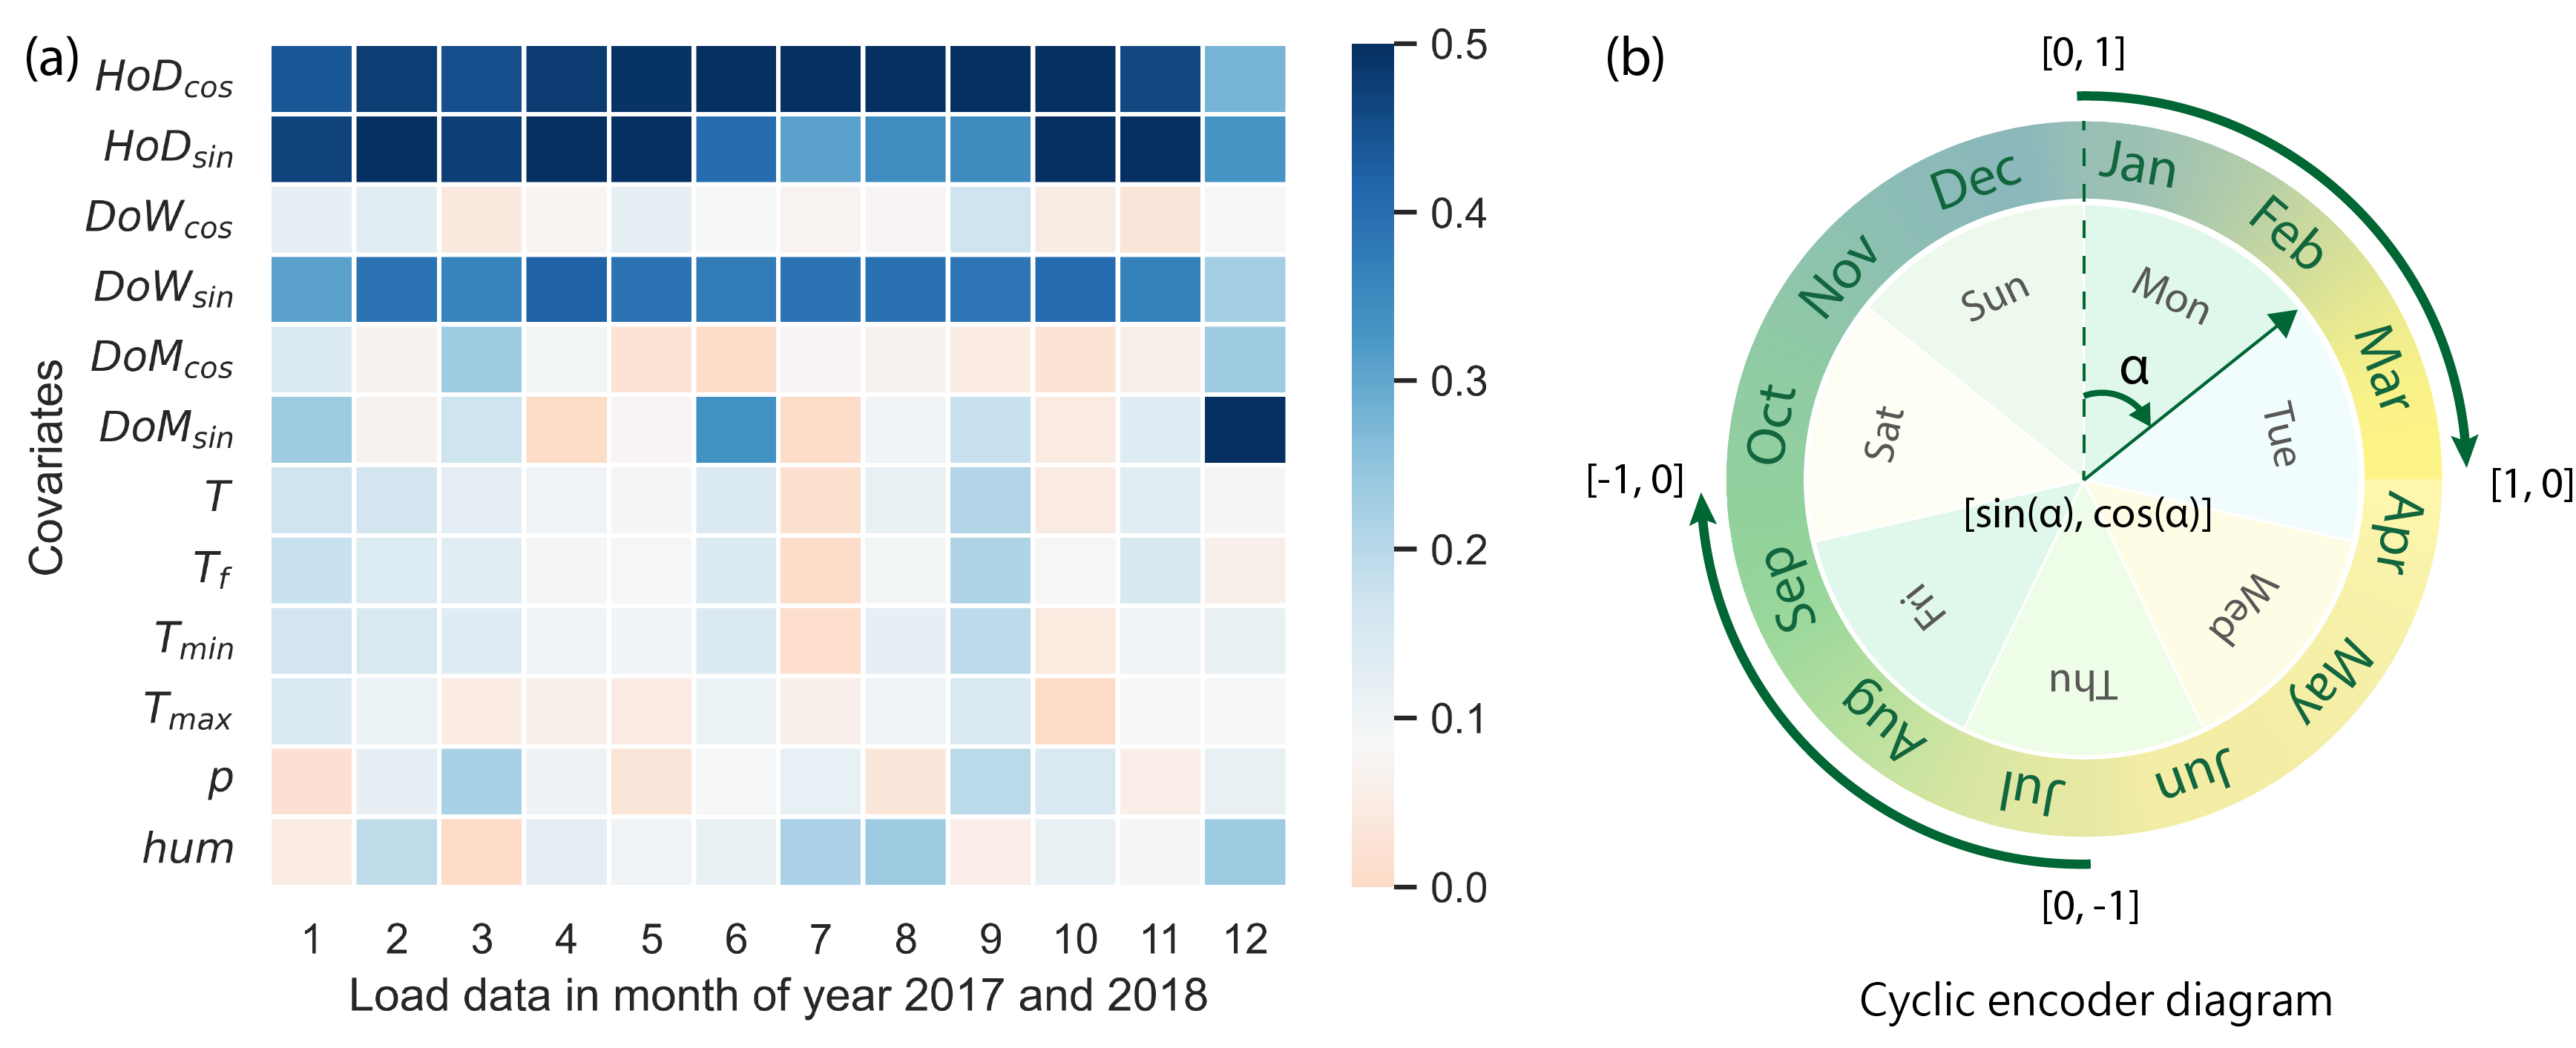
\includegraphics[width=0.85\textwidth]{figures/Pearson_correlation_and_cyclic.png}
  \caption{\textit{Pearson correlation and cyclic encoder diagram} \textbf{(a)}. Absolute Pearson correlation values between covariates and load data in a month. Month is given in $x$-axis and type of covariates labeled in $y$-axis. Deeper blue indicates higher value of correlation, and orange indicates value below 0.1. \textbf{(b)}. The diagram shows the encoding rule of cyclic encoding. For simplicity, only month of year (MoY) and day of week (DoW) are shown in the diagram. }
  \label{fig:pearson_cyclic}
\end{figure}


In the context of the forecasting tasks of this study, covariates pertain to external data that can be utilized as inputs for model enhancement seeking to improve forecasts. These external data encompass meteorological data ($\mathbf{CO^M}$) and time feature data ($\mathbf{CO^T}$).  The target to predict is the series of building loads, and the covariates themselves are not predicted. 

%\footnote{More information about meteorological data we used is provided in the Appendix. }
\emph{Meteorological data} was retrieved from \emph{OpenWeather} with an hourly granularity. The measured data includes: ambient air temperature ($\mathbf{T}$, ℃), feels-like temperature ($\mathbf{T_f}$, ℃), atmospheric pressure ($\mathbf{p}$, mmHg) and relative humidity ($\mathbf{hum}$, \%). Having perceived that the daily load patterns of the profile are associated with the activity intensity during workday or holiday, we encode \emph{time feature} covariates including hour of day ($\mathbf{HoD}$), day of week ($\mathbf{DoW}$), month of year ($\mathbf{MoY}$) and day of month ($\mathbf{DoM}$). These inputs use a cyclic encoder (see Fig. \ref{fig:pearson_cyclic}-\textbf{b}), which can help the model describe the periodic temporal features more objectively compared with the integer and one-hot approaches\cite{cyclic_encode}. Furthermore, a boolean variable ($\mathbf{D_{work}}$) is included to indicate whether the day is a workday.

As shown in Fig. \ref{fig:pearson_cyclic}-\textbf{a}, most covariates we selected have correlation value higher than 0.1. Among all covariates, time features, particularly $\mathbf{HoD}$ and $\mathbf{DoW}$, show strong relations with monthly load data. Although \emph{meteorological data} has limited correlation with load data, it still provide information which can be useful for forecasting in several months. 

%\footnote{Every four sets of building load and PV generation data within an hour share the same set of meteorological data, aligning both datasets into time series with a frequency of 15 minutes for future training purposes.}
%\footnote{Three sub variables are provided in the dataset: maximum, minimum and average ambient air temperature in the measuring period (an hour). }
%\footnote{Feels like temperature accounts for human perception of weather, and it is calculated using the following formula: $\mathbf{T_f}$ = $Ta$ + 0.33$\rho$ - 0.7$ws$ - 4, where $Ta$ is the dry bulb temperature (℃), $\rho$ is the water vapor pressure (hPa) and $ws$ is the wind speed (m/s) at 10 meter above the ground.\cite{steadman1994norms}}
%\footnote{\emph{OpenWeather} is a provider of high accuracy weather data which sourced from weather stations, weather radar data and satellite data. }

%In forecasting models' training and testing stages, covariates are classified as two types: past covariates known only in the past and future covariates known in the future. As the meteorological data used are measured values instead of forecasts, it functions as only past covariates. Time features can work as both past and future covariates naturally, as they can be predetermined.


\subsubsection{Linear regression (LR)}
% Machine learning - Linear Regression

\begin{figure}[!ht]
\centering
  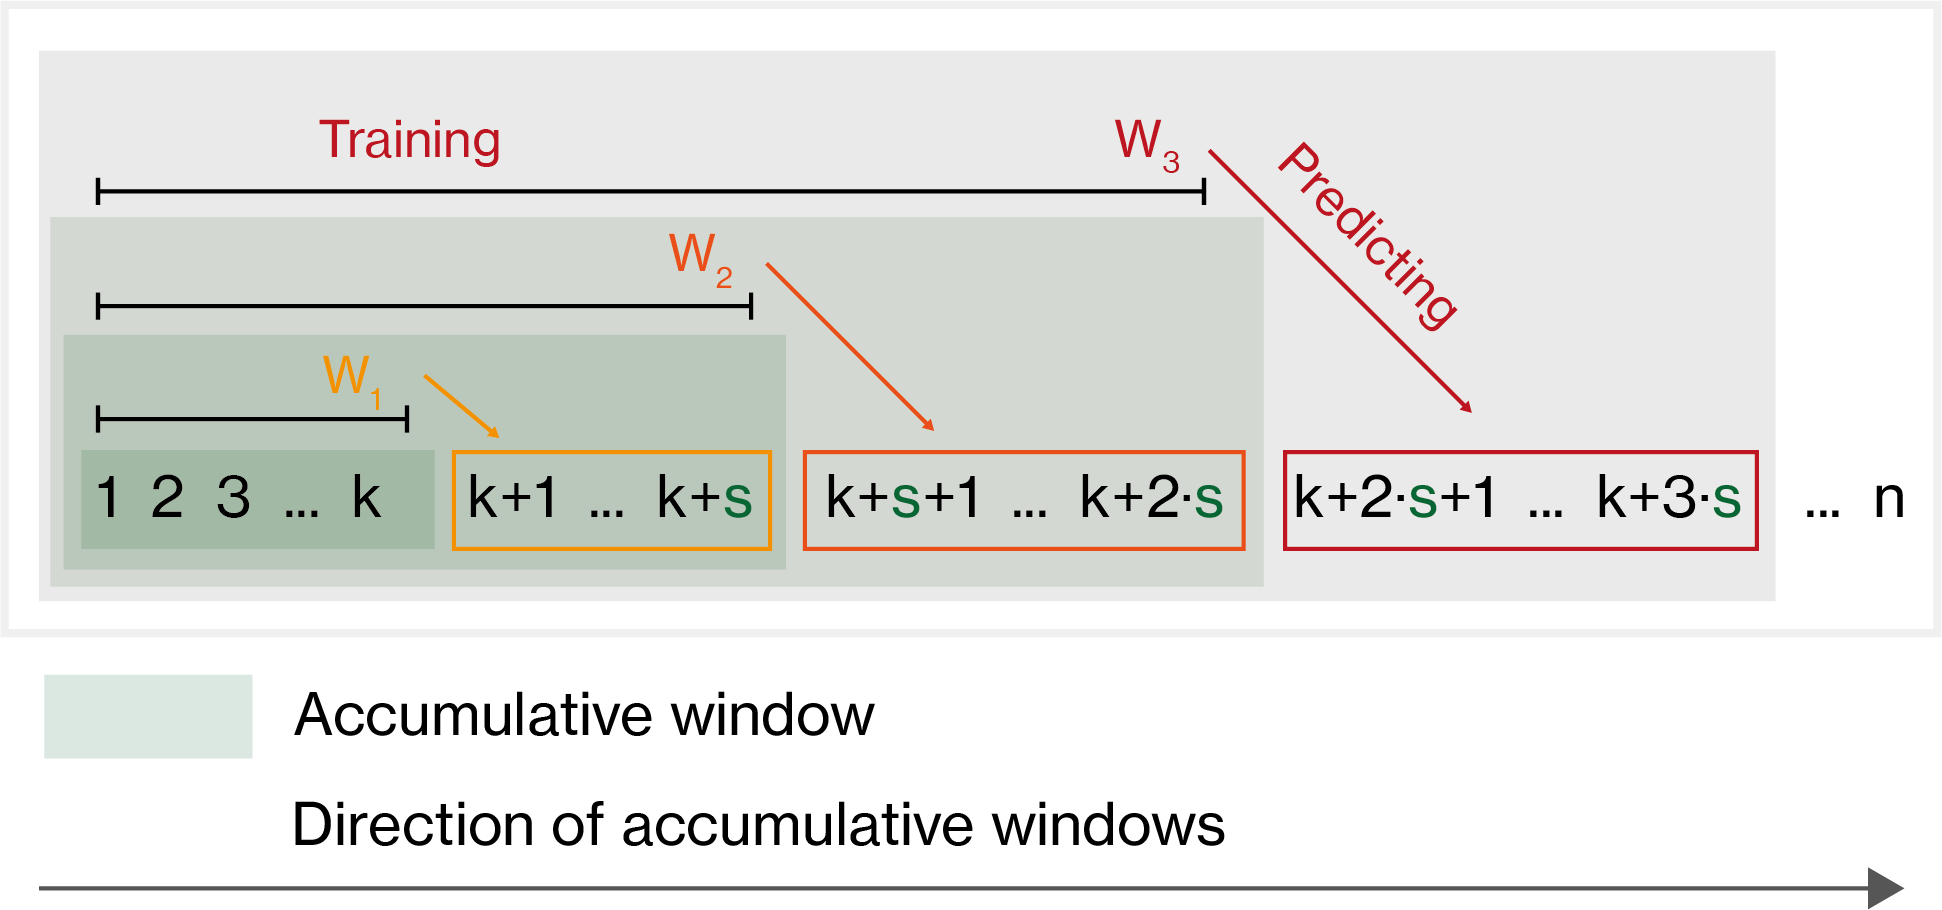
\includegraphics[width=0.55\textwidth]{figures/Accumulative retraining.png}
  \caption{\textit{Accumulative training diagram.} $W$ represents the windows for each training, $s$ is the prediction steps. In this study, the initial $W_1$ is 61080 steps (data of year 2017 and 2018) and $s$ is 96 steps (data of one day). }
  \label{fig:Accumulative}
\end{figure}

Linear regression is a statistical modeling technique used to establish a linear relationship between a dependent variable and one or more independent variables. It assumes a linear relationship between the variables and aims to find the best-fit line that minimizes the difference between the predicted values and the actual values. Linear regression is widely used for forecasting and prediction tasks because of its capability to achieve reliable predictive performance and cross-compatibility\cite{city_scale_pred}, especially when the relationship between the variables is believed to be linear. Compared with other complicated machine learning techniques, training a LR model is fast, even when dealing with large data sets. Thus, online forecasting is feasible, which is also known as accumulative training. The process of accumulative training is shown in Fig. \ref{fig:Accumulative}. This method gradually expands the size of training data without overflowing historical data. Increasing training data can reduce the prediction errors\cite{online_LR}. We denote MPC with forecasts generated by this method as \textbf{MPC-LR}. Furthermore, we execute an additional forecasting technique utilizing LR by incorporating covariates namely time characteristics and meteorological data. The designation for MPC utilizing this forecast is \textbf{MPC-LRCo}.

\subsubsection{Probabilistic forecasting with autoregressive recurrent networks (DeepAR)}
% Machine learning - Probabilistic forecasting with autoregressive recurrent networks

Probabilistic forecasting with autoregressive recurrent networks (DeepAR) is a method that combines autoregressive models and recurrent neural networks (RNNs) to make probabilistic predictions. In some cases, long short-term memory (LSTM) can be used to replace the RNN. AR models capture dependencies between past and current observations, while RNNs are designed to model sequential data. By combining these two techniques, probabilistic forecasting with AR networks can generate predictions along with a measure of uncertainty, providing a probabilistic distribution of future values. DeepAR is good at learning seasonal behaviors and dependencies on given covariates across time series. At the same time, little manual intervention in providing covariates is needed in order to capture complex behaviors\cite{DeepAR}. In this method, only future covariates (i.e. time features) are encoded due to the limitation of RNN model. MPC with this prediction is denoted as \textbf{MPC-DeepAR}.

\subsubsection{Temporal Fusion Transformer (TFT)}
% Machine learning - Temporal fusion transformer

The Temporal Fusion Transformer (TFT) is a forecasting model that combines elements of recurrent neural networks and transformers. It is designed to capture complex temporal patterns in time series data. TFT uses a hierarchical architecture that includes encoder-decoder layers, attention mechanisms, and gating mechanisms. It can handle multiple time series inputs and can model long-range dependencies effectively. TFT has been shown to deliver accurate and interpretable predictions for various forecasting tasks\cite{TFT}. Major constituents of TFT related to our forecasting task include gating mechanisms, variable selection networks and temporal processing. Gating mechanisms and variable selection networks help select relevant input variables at each time step. In the temporal processing mechanism, a sequence-to-sequence layer is employed for local processing of short-term dependencies, while long-term temporal relations are captured using a novel interpretable multi-head attention block.  MPC with this prediction is denoted as \textbf{MPC-TFT}.

\subsubsection{Extreme Gradient Boosting (XGBoost)}
% Machine learning - Extreme gradient boosting 

Extreme Gradient Boosting (XGBoost) is a popular machine learning algorithm known for its efficiency and predictive power. XGBoost is an ensemble method that combines multiple weak prediction models, typically decision trees, into a strong predictive model. It uses gradient boosting, which sequentially trains models by focusing on the errors made by previous models \cite{XGBoost}. XGBoost incorporates regularization techniques to prevent overfitting and provides high accuracy for various prediction tasks, including regression and classification. XGBoost is widely used for building-scale\cite{wang2020building} and city-scale\cite{wang2021predicting} load forecasting, and is also a frequent winner in Kaggle forecasting competitions\cite{Kaggle}. Its performance mainly attributes to these innovations: the tree-learning algorithm boosting sparse data process, a theoretically justified weighted quantile sketch procedure enabling approximate tree learning, and parallelisation together with distributed computing shrinking the training time. Benefited by the tree-learning algorithm, both meteorological and time feature covariates are utilized in XGBoost training. MPC with this prediction is denoted as \textbf{MPC-XGBoost}.

\subsubsection{Hyperparameter tuning}

For machine learning tasks, hyperparameter searching is a cumbersome and time consuming process. Due to model complexity and large size of training data, conventional grid-search approach is not applicable in this study. Thus we chose \textit{Optuna}, an efficient way of hyperparameter tuning adopting efficient searching and pruning algorithms\cite{optuna_2019}, as our hyperparameter tuning method. Corresponding configurations for DeepAR, TFT and XGBoost are listed in Table. \ref{tab:Optuna}.

\begin{table}\centering
\renewcommand\arraystretch{1} %行高为1.5倍
\setlength{\abovecaptionskip}{10pt}
\setlength{\belowcaptionskip}{-10pt}
\begin{tabular}{cccc}
   \toprule
   % & T & Models &  &  \\
   Model parameters & TFT & DeepAR & XGBoost   \\
   \midrule
   used covariates & $CO^T$ & $CO^T$ & $CO^T$, $CO^M$  \\ 
   epochs & [1, 100] & [1, 50] & [1, 250]   \\
   optimization trials & 100 & 100 & 30   \\
   learning rate & [$10^{-4}$, 1] & [$10^{-4}$, 1] & [$10^{-3}$, 1] \\
   batch size & 96 & [8, 672] & - \\
   dropout rate & [0.01, 1] & [0.01, 1] & - \\
   \midrule
   % input chunk length & 672 & 672 & - \\
   % output chunk length & 96 & 96 & - \\
   % gradient clip & 0.1 & 0.1 & - \\
   RNN layers & - & [1, 8] & - \\
   \midrule
   LSTM layers & [1, 8] & - & - \\
   hidden dimensions & [1, 8] & - & - \\
   attention heads & [1, 8] & - & - \\
   \midrule
   minimum child weight & - & - & [5, 10] \\
    maximum depth& -& -&[1, 5]\\
    gamma& -& -&[0.25, 1]\\
    subsample  & -& -&[0.01, 0.2]\\
    colsample bytree& -& -&[0.01, 0.2]\\
    regularization alpha& -& -&[$10^{-8}$, 1]\\
    regularization lambda& -& -&[$10^{-8}$, 1]\\
    \bottomrule
\end{tabular}
\caption{Hyperparameters for \emph{Optuna} searching}\centering
    \label{tab:Optuna}
\end{table}


\subsubsection{Adaptive moving average (AMA)}

In contrast with \emph{machine learning} approaches, \emph{heuristic} methods are simple and intuitive. We adopt a quite simple heuristic model for building load forecast. Specifically, the estimate for time step $t+k$ forecast at time $t$:
\begin{equation}
    \bldest_{t+k \mid t} = \alpha^k \pbld_{t-1} + (1 - \alpha^k) \bldavg_{\tset(t+k)} 
\end{equation}
where $\bldavg_{\mathcal{A}} = \frac{1}{\abs{\mathcal{A}}}\sum_{t\in \mathcal{A}} \pbld_t$ is the average of some selected historical data, and for our specific choice, $\tset(t)$ is the set of the most recent four steps whose day-of-week (DoW) and time-of-day (ToD) are the same as $t$. We pick $\alpha = 0.1$. 
Since it combines last observed data with exponentially decaying historical data as the prediction window moving forward, we call this implementation as adaptive moving average (AMA). MPC with this prediction is denoted as \textbf{MPC-AMA}.

% The overall prediction MAPE is 6.63\% in 2019.\footnote{Our model is adaptive since we include the last time step $\pbld_{t-1}$ as a reference, which is usually good estimate for very near future. MAPE for $k\le 4$ is 3.13\%, while MAPE for $48 < k\le 96$ is 6.90\% (1 hour contains 4 steps).} 

\subsubsection{Forecast accuracy}
    
The forecasting performances are primarily evaluated by using four (lump) metrics, as defined in Eqs. \eqref{eq:MAE}-\eqref{eq:CV-RMSE}, where $y_t$ and $\widehat{y_t}$ are actual and forecasting values. They are the mean absolute error (MAE), the root mean squared error (RMSE), the mean absolute percentage error (MAPE) and the coefficient of variation of the root mean squared error (CV-RMSE). MAE and RMSE are scale-dependent which can provide a straight-forward quantification to the readers, while MAPE and CV-RMSE are normalized metrics so it is more comparable across specific buildings. In addition, existing studies and guidelines provided some benchmarks for evaluating the model by using CV-RMSE. Specifically, resulting CV-RMSE below 30\% indicates the model is calibrated and sufficiently close to physical reality for engineering purposes when using hourly data\cite{CV-RMSE_standard}.  

\begin{figure}[!ht]
\centering
  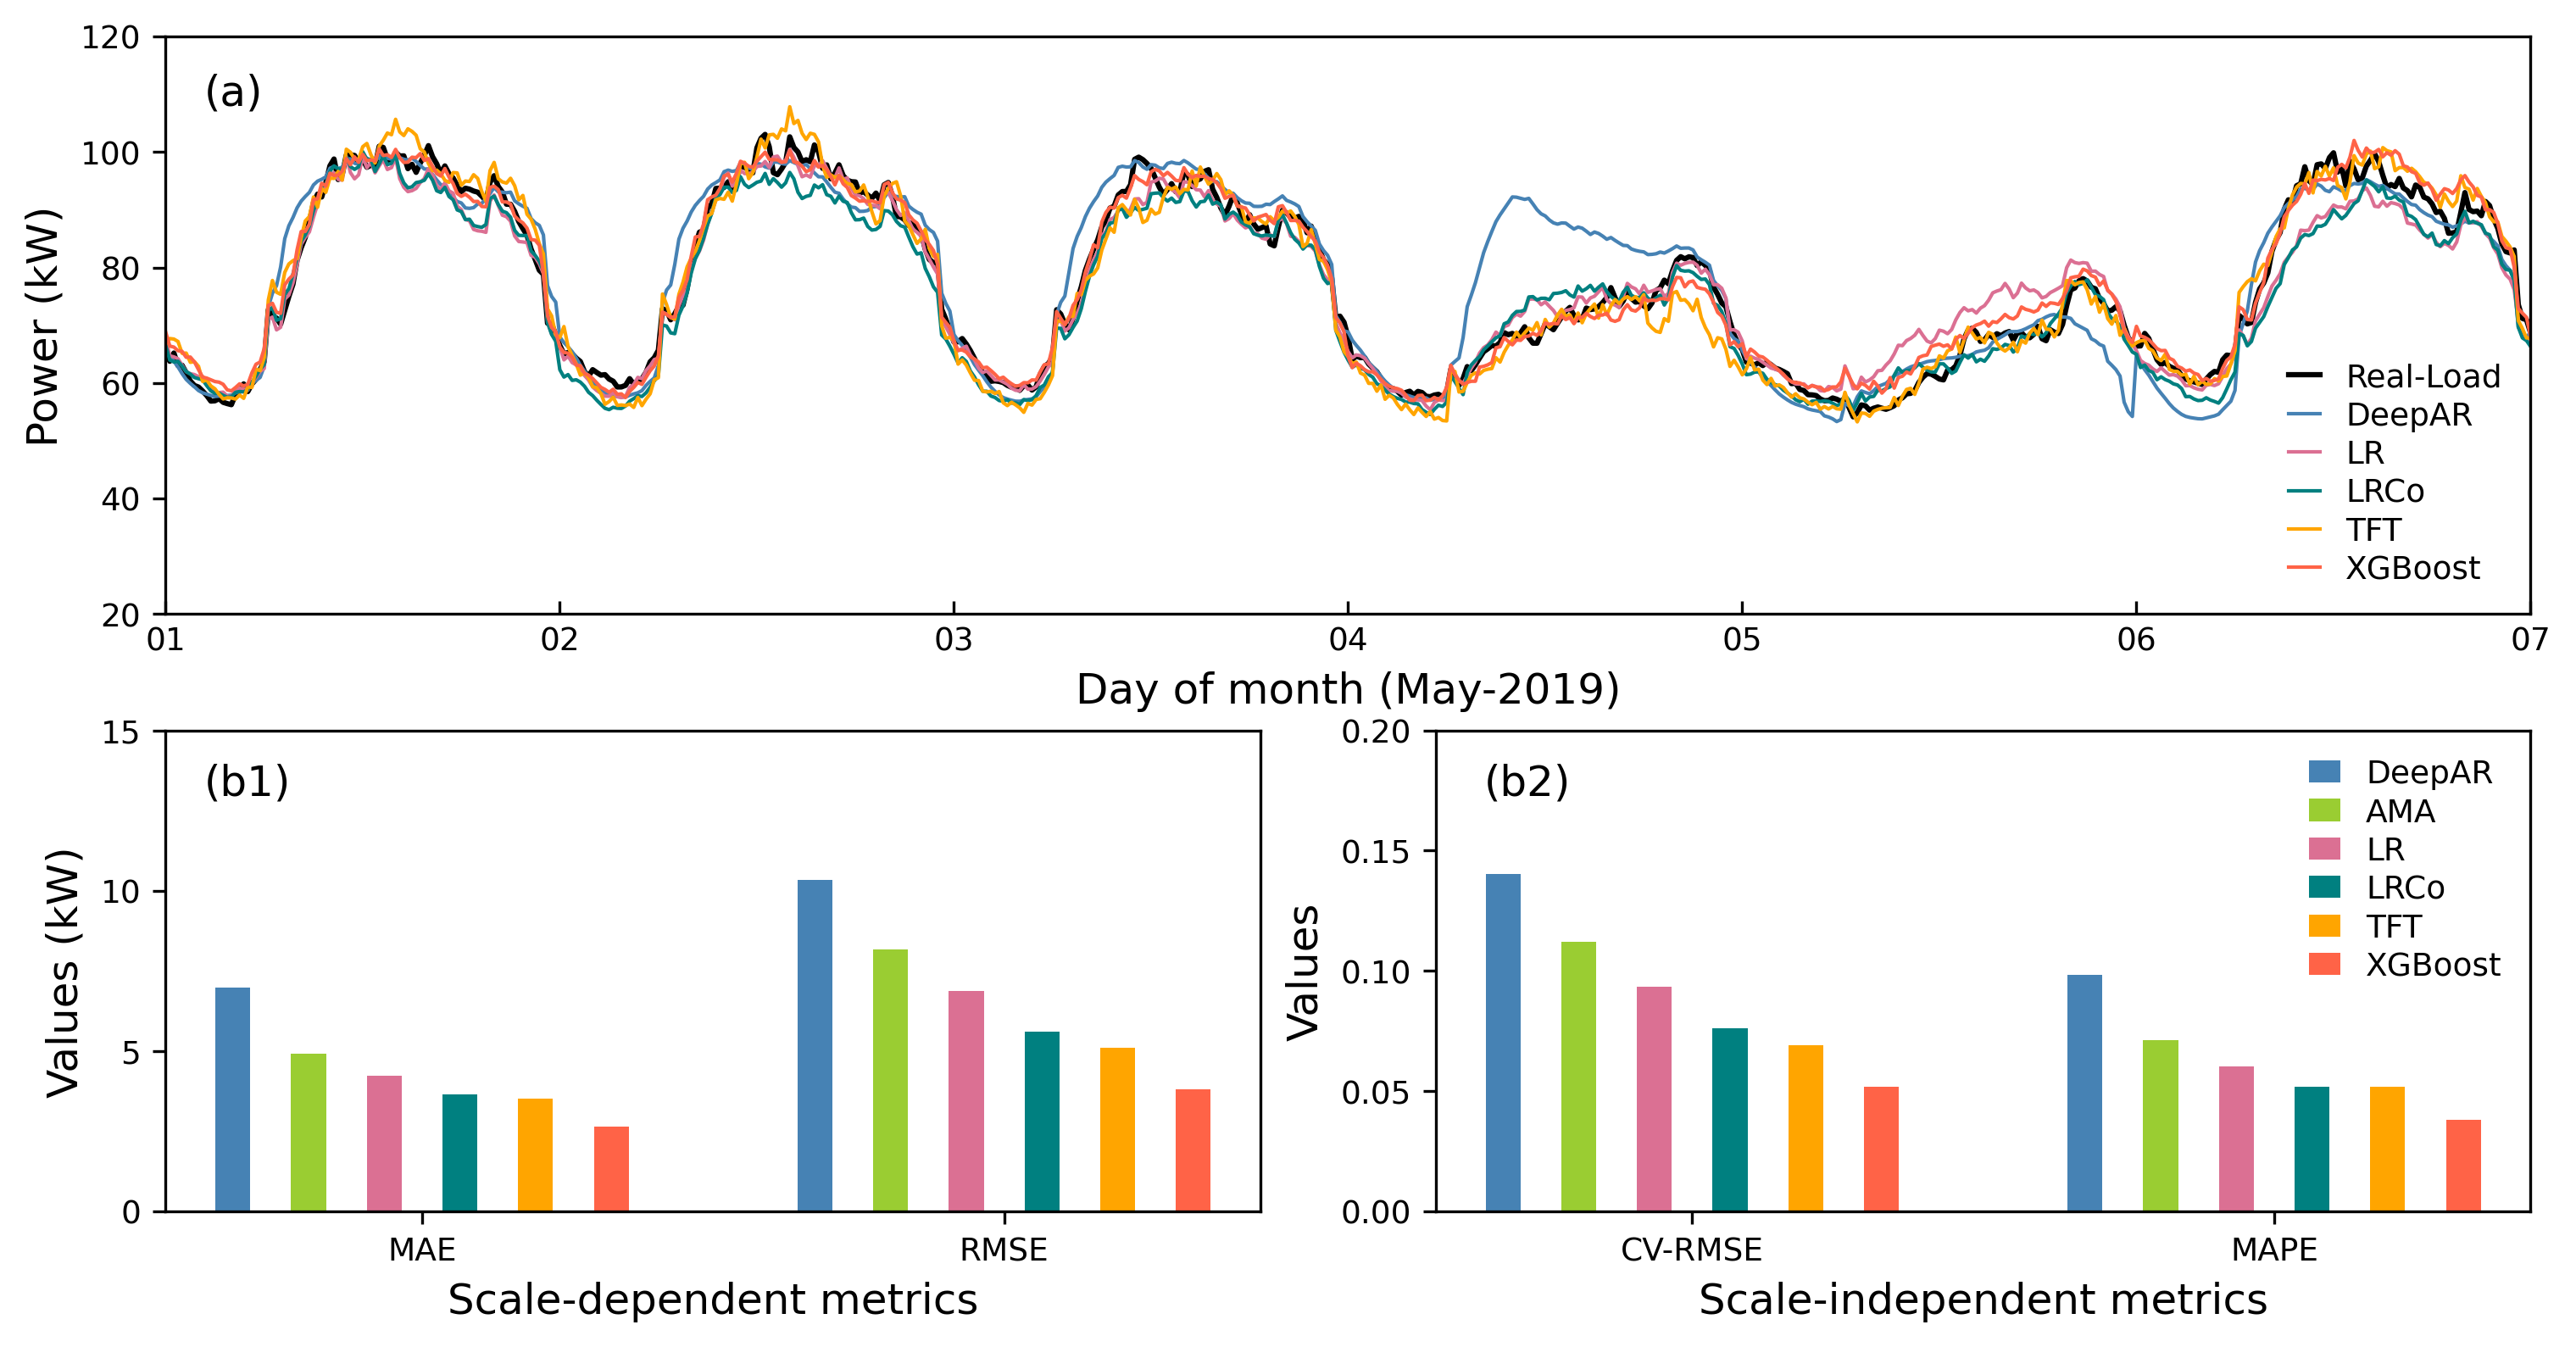
\includegraphics[width=0.85\textwidth]{figures/fig-1-load-prediction-and-metrics.png}
  \caption{\textit{Sample forecasts and error metrics} \textbf{(a)}. Real load values are represented by black line, and forecasts of different machine learning models are colored lines as tagged in legend. The AMA generates adaptive forecasts, which are not plotted in this figure. \textbf{(b1)-(b2)} Visualizing the scale-dependent and scale-independent metrics of different forecasts. }
  \label{fig:prediction}
\end{figure}

\begin{equation} \label{eq:MAE}
    MAE = \frac{1}{n} \sum_{t=1}^{n}\abs{y_{t}-\widehat{y_{t}}}
\end{equation}

\begin{equation}
    RMSE = \frac{1}{n} \sqrt {\sum_{t=1}^{n}(y_{t}-\widehat{y_{t}})^{2}}
\end{equation}

\begin{equation}
    MAPE = \frac{1}{n}\sum_{t=1}^{n} \abs{\frac{y_t-\widehat{y}_t}{y_t}}
\end{equation}
    
\begin{equation} \label{eq:CV-RMSE}
    CV-RMSE = \frac{\sqrt{\frac{\sum_{t=1}^{n}(y_{t}-\widehat{y_{t}})^{2}}{n}}} {\frac{\sum_{t=1}^{n} y_{t}}{n}}
\end{equation}

%\lunlong{Explanations for forecasting results will be added.}
  
% \lunlong{Maybe the explanation of OPEX, TOU should be placed here?}
%In this paper, we denote the set of real numbers by $\R$ and the set of integers by $\Z$. We use functions $\ind{\cdot}$, $[\cdot]^{+}$, $[\cdot]^{-}$, $\lfloor \cdot \rfloor$ in their conventional meanings, i.e., $\ind{x}=1$ if $x$ is true otherwise $\ind{x}=0$, $[x]^{+} \coloneqq \max\{0,x\}$, $[x]^{-} \coloneqq \min\{0,x\}$.\footnote{For consistency, we adopt the convention that using lowercase letters (e.g., $x$) for (decision) variables, uppercase letters (e.g., $X$) and Greek letters (e.g., $\alpha$) for parameters, and calligraphic uppercase letters (e.g., $\mathcal{X}$) for sets.}
Fig. \ref{fig:prediction}. provides sample forecasts of a week, and summarizes the resulting MAE, RMSE, CV-RMSE and MAPE. In general, all forecasting models outperform the threshold of 30\% in terms of CV-RMSE, showcasing a range from 5.17\% to 14.04\%. Compared to performances provided by other related research \cite{hourly_building_cooling_load_pred}, the resulting CV-RMSE is lower. This enhanced performance can be attributed to the nature of the building load data employed in this study, which represents the average demand of eight individual buildings. This aggregation serves to mitigate the inherent uncertainty in load patterns, resulting in more robust forecasting outcomes.
Among all accessed methods, XGBoost emerges as the frontrunner, exhibiting superior performance with a MAPE of 3.80\%. TFT has the resulting MAPE of 5.19\% inferior to XGBoost. Though the structure of LR is rather simple, it exerts good performance of 6.01\% (MAPE), as a result of constantly retraining. By encoding covariates, the MAPE of LRCo is enhanced to 5.18\%. Of particular note is the heuristic method AMA, which defies expectations with its robust performance, despite its simplicity. Leveraging observations from the preceding time step, AMA attains a MAPE of 7.13\%, surpassing the performance of the more intricate DeepAR model, which registers a MAPE of 9.83\%.

%============================================================================================================
\subsection{Simulation configurations}
\label{section:configurations}
Based on streamed PV and building load data and corresponding forecasts in the year of 2019, the simulations are performed under two scenarios ($\wodc$ and $\wdc$) to examine the impact of pricing schemes. Under $\wodc$ (without demand charge), the utility bills consists of only TOU (time of use) costs, where the demand charge rate $\dc$ was set as $0$ \$/kW. Under $\wdc$ (with demand charge), the demand charge rate $\dc$ was set as $18$ \$/kW in a billing cycle of one month, representing a typical scenario in California. Apart from the demand charge rate $\dc$, other configurations for both scenarios are set as follows: 
 
In order to make our analysis more generalizable, we intentionally rescaled the annual PV generation and the battery capacity, then they are proportional to the annual building load. The factors, namely $\rpv$ and $\rbat$ were set as 50\% and 6h in this study. Battery (dis)charging efficiencies were set as $0.98$. 
We used the day-ahead price (DA) of San Diego Gas \& Electric (SDGE) as the grid TOU $\tou^+$\footnote{Considering the price difference between wholesale markets and business plans, we rescaled TOU so that its average was $0.17$ \$/kWh. We assume DA is known.}. Selling prices $\tou^-$ were set as fixed proportion to buying prices $\tou^+$, and the factor was $0.6$ in our base case.
%============================================================================================================

\section{Results} \label{sec:results}

%\newcommand{\bldavg}{\overline{P}^{\text{D}}}
\newcommand{\noise}{\mathbf{U}}
\newcommand{\noisePos}{\mathbf{U^+}}
\newcommand{\noiseNeg}{\mathbf{U^-}}

%\lunlong{Captions of figures are not revised.}

\subsection{The impact of pricing schemes}
    \label{sec:Polarized accuracy}

The first finding of this study reveals that the performance of MPC varies under different pricing schemes, namely $\wodc$ and $\wdc$, despite having the same forecast. Under $\wodc$, enhancing forecast accuracy does not yield equitable progress for MPC in terms of VoI*. And MPC with inferior forecasts attains near optimal control performance. In contrast, under $\wdc$, MPC with highly precise forecasts exhibits VoI* that is inferior compared to RBC. 


\begin{figure}[!ht]
\centering
  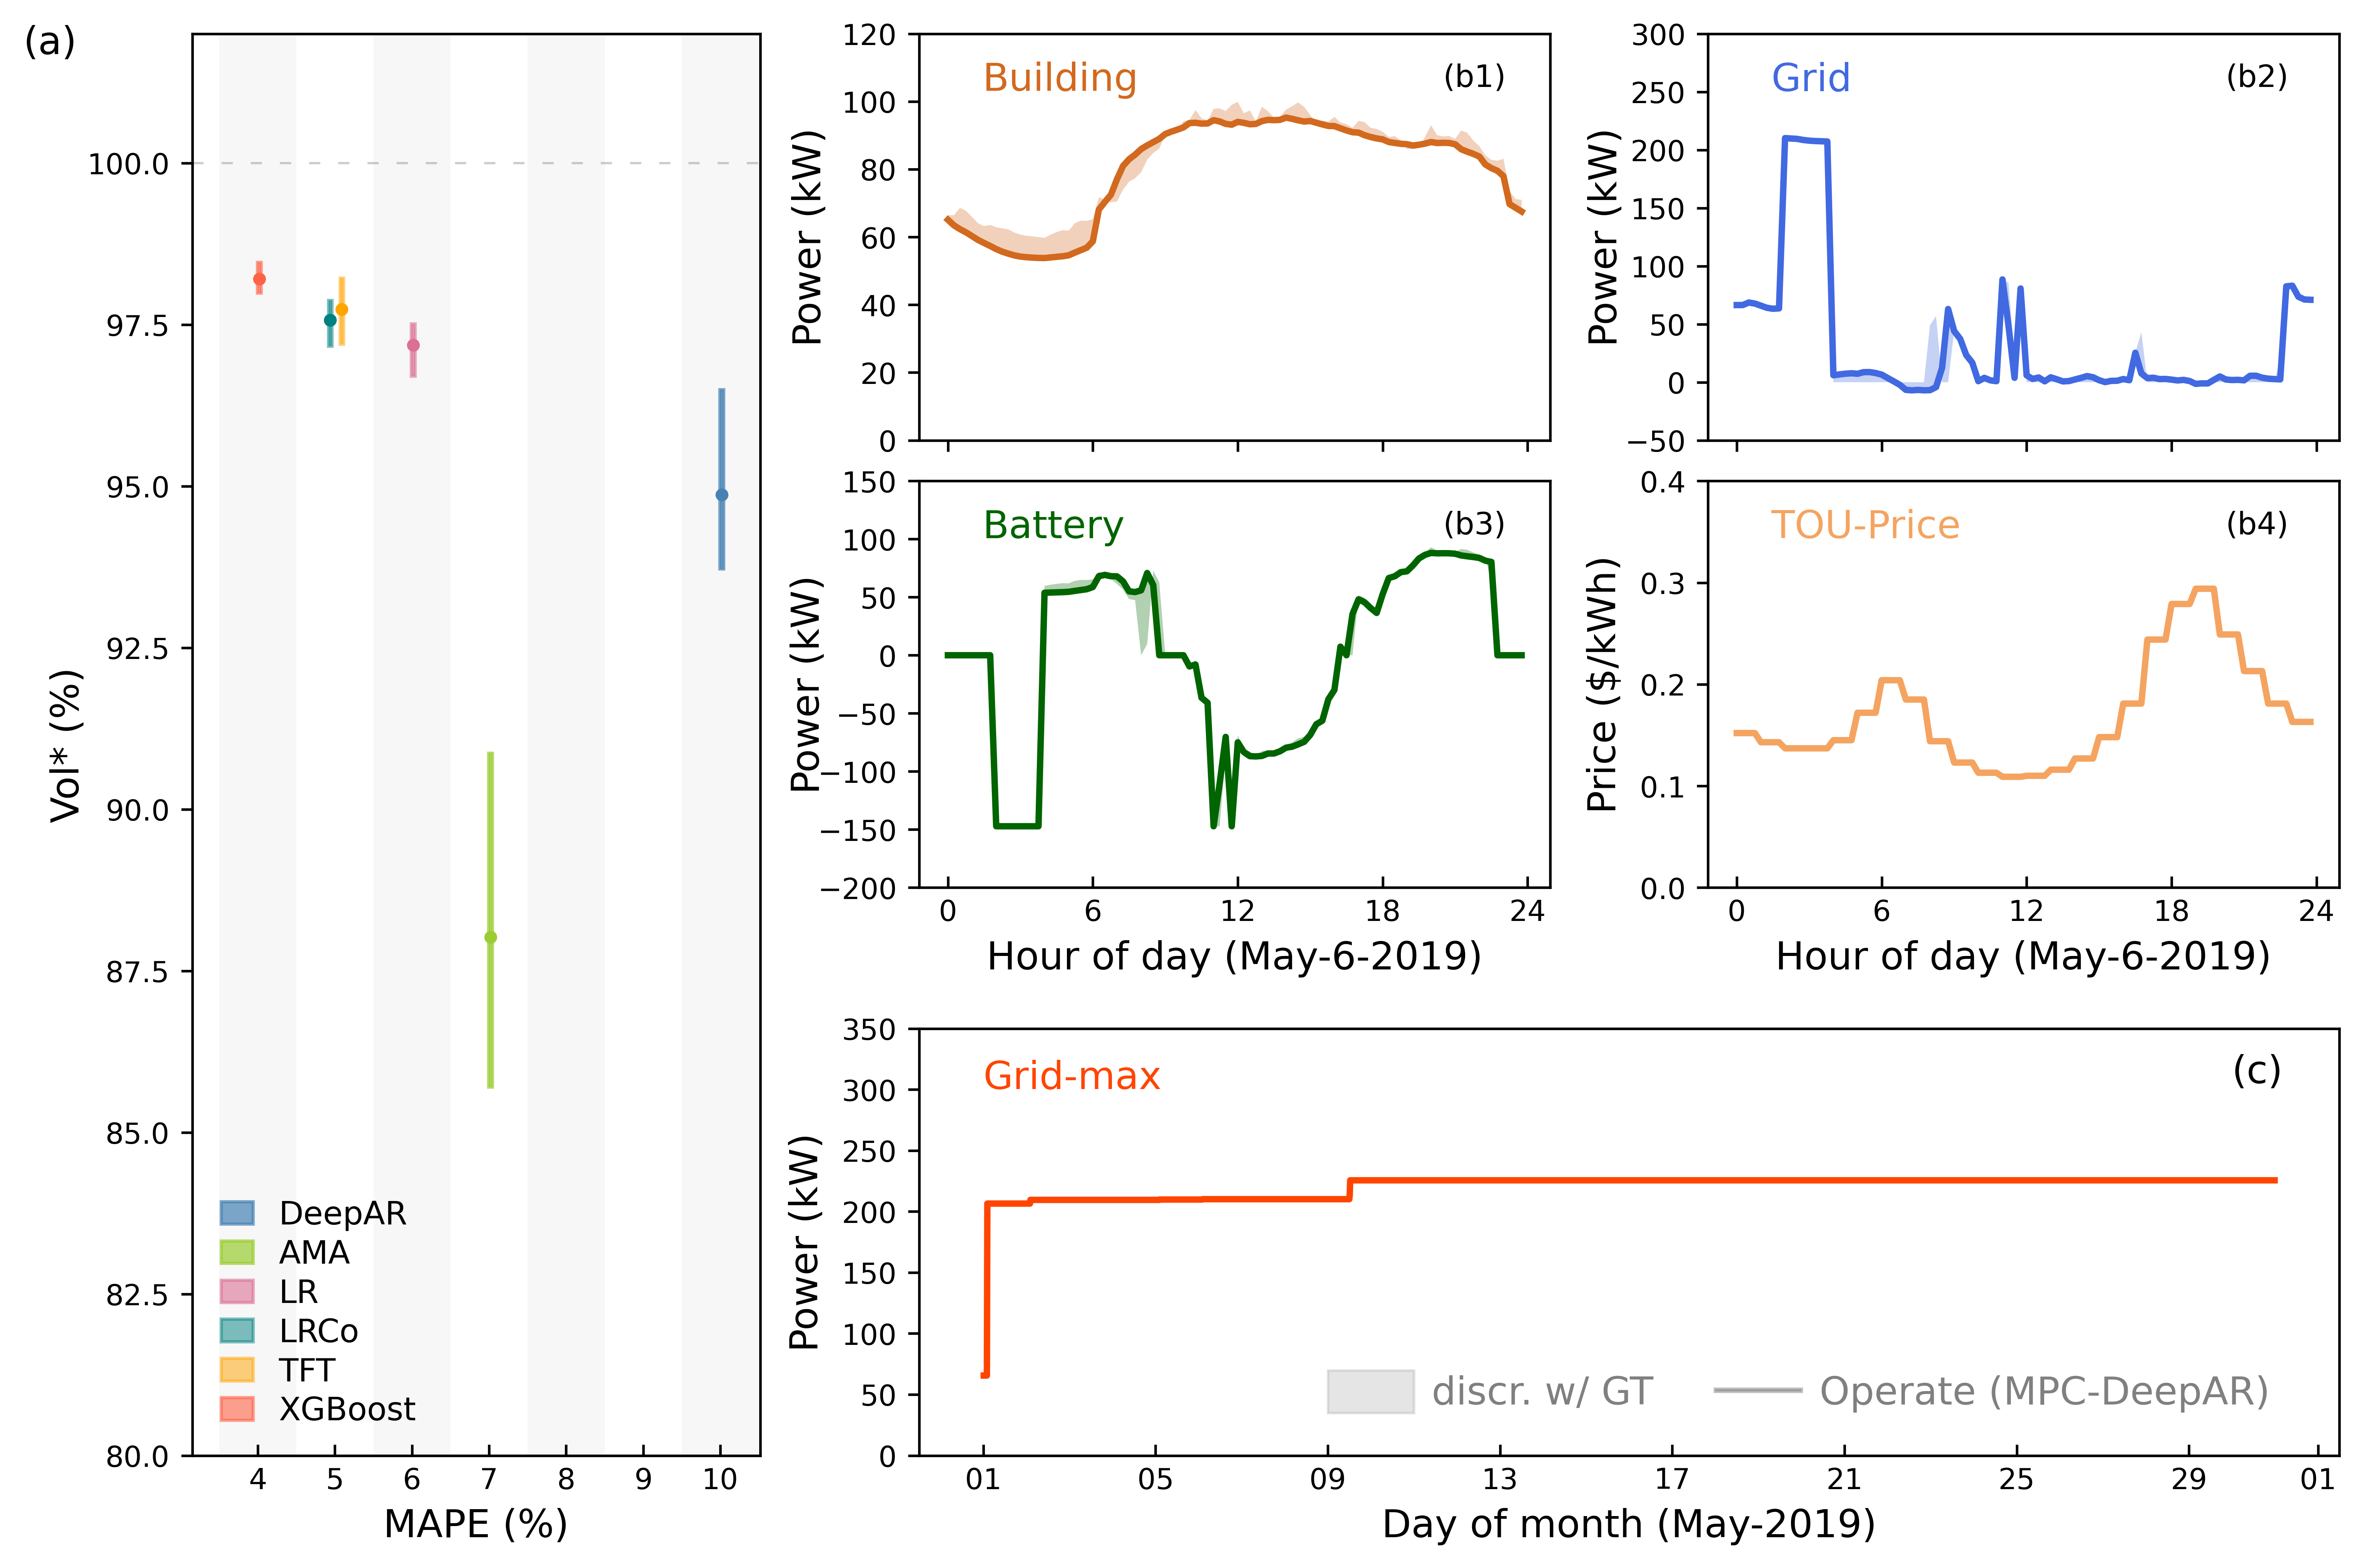
\includegraphics[width=0.75\textwidth]{figures/fig-2-without-dc-2.png}
  \caption{\textit{Control performance and sample control sequences under $\wodc$.} \textbf{(a)} Performance of MPC with all available predictions as stated in previous sections. $x$-axis shows the forecasting error (MAPE), and $y$-axis is the corresponding normalized value of information (VoI*). Each bar marks the 25\% and 75\% percentiles of trials for 12 months of 2019. \textbf{(b1)-(b4)} Sample control sequences of \textbf{MPC-DeepAR}. \textbf{(c)} Peak imported power tracking till the moment. (In (b1)-(b4) and (c), solid line represents actions that are actually executed, and shaded area shows discrepancy between executed actions and optimal actions by MPC-GT. For building, shaded area means prediction error.) }
  \label{fig:group-plot-0dc}
\end{figure}

\textbf{Under \texorpdfstring{$\wodc$}{Lg}}

Fig. \ref{fig:group-plot-0dc} presents the quantified control performance and sample control sequences under $\wodc$. Fig. \ref{fig:group-plot-0dc}-\textbf{a} gives the performance of MPC with all forecasts, whose prediction errors (MAPE) vary significantly, ranging from 3.8\% (XGBoost) to 9.83\% (DeepAR). The control performances for the majority of monthly trials achieved near-optimal levels of VoI* around 90\%.

Fig. \ref{fig:group-plot-0dc}-\textbf{b1} to \textbf{b4} present control sequences of \textbf{MPC-DeepAR}, which demonstrate near-identical control behaviors to the optimal ones. The TOU tariff peaks at around 7:00 and 19:00, when the external grid importation is decreased to almost zero by using the BESS as a substitute, which was charged beforehand during low-TOU-tariff periods. Throughout the process, the shaded area in Fig. \ref{fig:group-plot-0dc}-\textbf{b1}. demonstrates that the forecast errors do not result in significant sub-optimality. This suggests that the forecasts provide ample information for the CFTOC problem to effectively utilize the gap between peak and valley of TOU tariff, thereby reducing the utility cost to near-optimal levels.

Under the $\wodc$ scenario, enhancing the forecast accuracy does not result in significant control performance enhancement. Despite reducing the MAPE from 9.83\% (DeepAR) to 3.80\% (XGBoost), the average VoI* increased by only 3.34\% from an already high level of 94.87\% to 98.21\%. 
Furthermore, compared to machine learning approaches, AMA is an ideal method for obtaining the near-future loads forecasts under $\wodc$. Since AMA requires limited historical data\footnote{Typically, utilizing data from the previous month is sufficient for achieving relatively accurate forecasts.} and is computationally efficient. It can be easily implemented whilst exhibiting a strong performance of 87.9\% with respect to VoI*.

%Considering computation complexity and historical data demand, AMA, the heuristic approach we proposed, is an optimal method for obtaining the near-future load prediction required for microgrid management. It can be easily implemented and requires only a short period of historical data whilst still exhibiting a strong performance of 87.9\% with respect to VoI*.

\textbf{Under \texorpdfstring{$\wdc$}{Lg}}

\begin{figure}[!ht]
\centering
  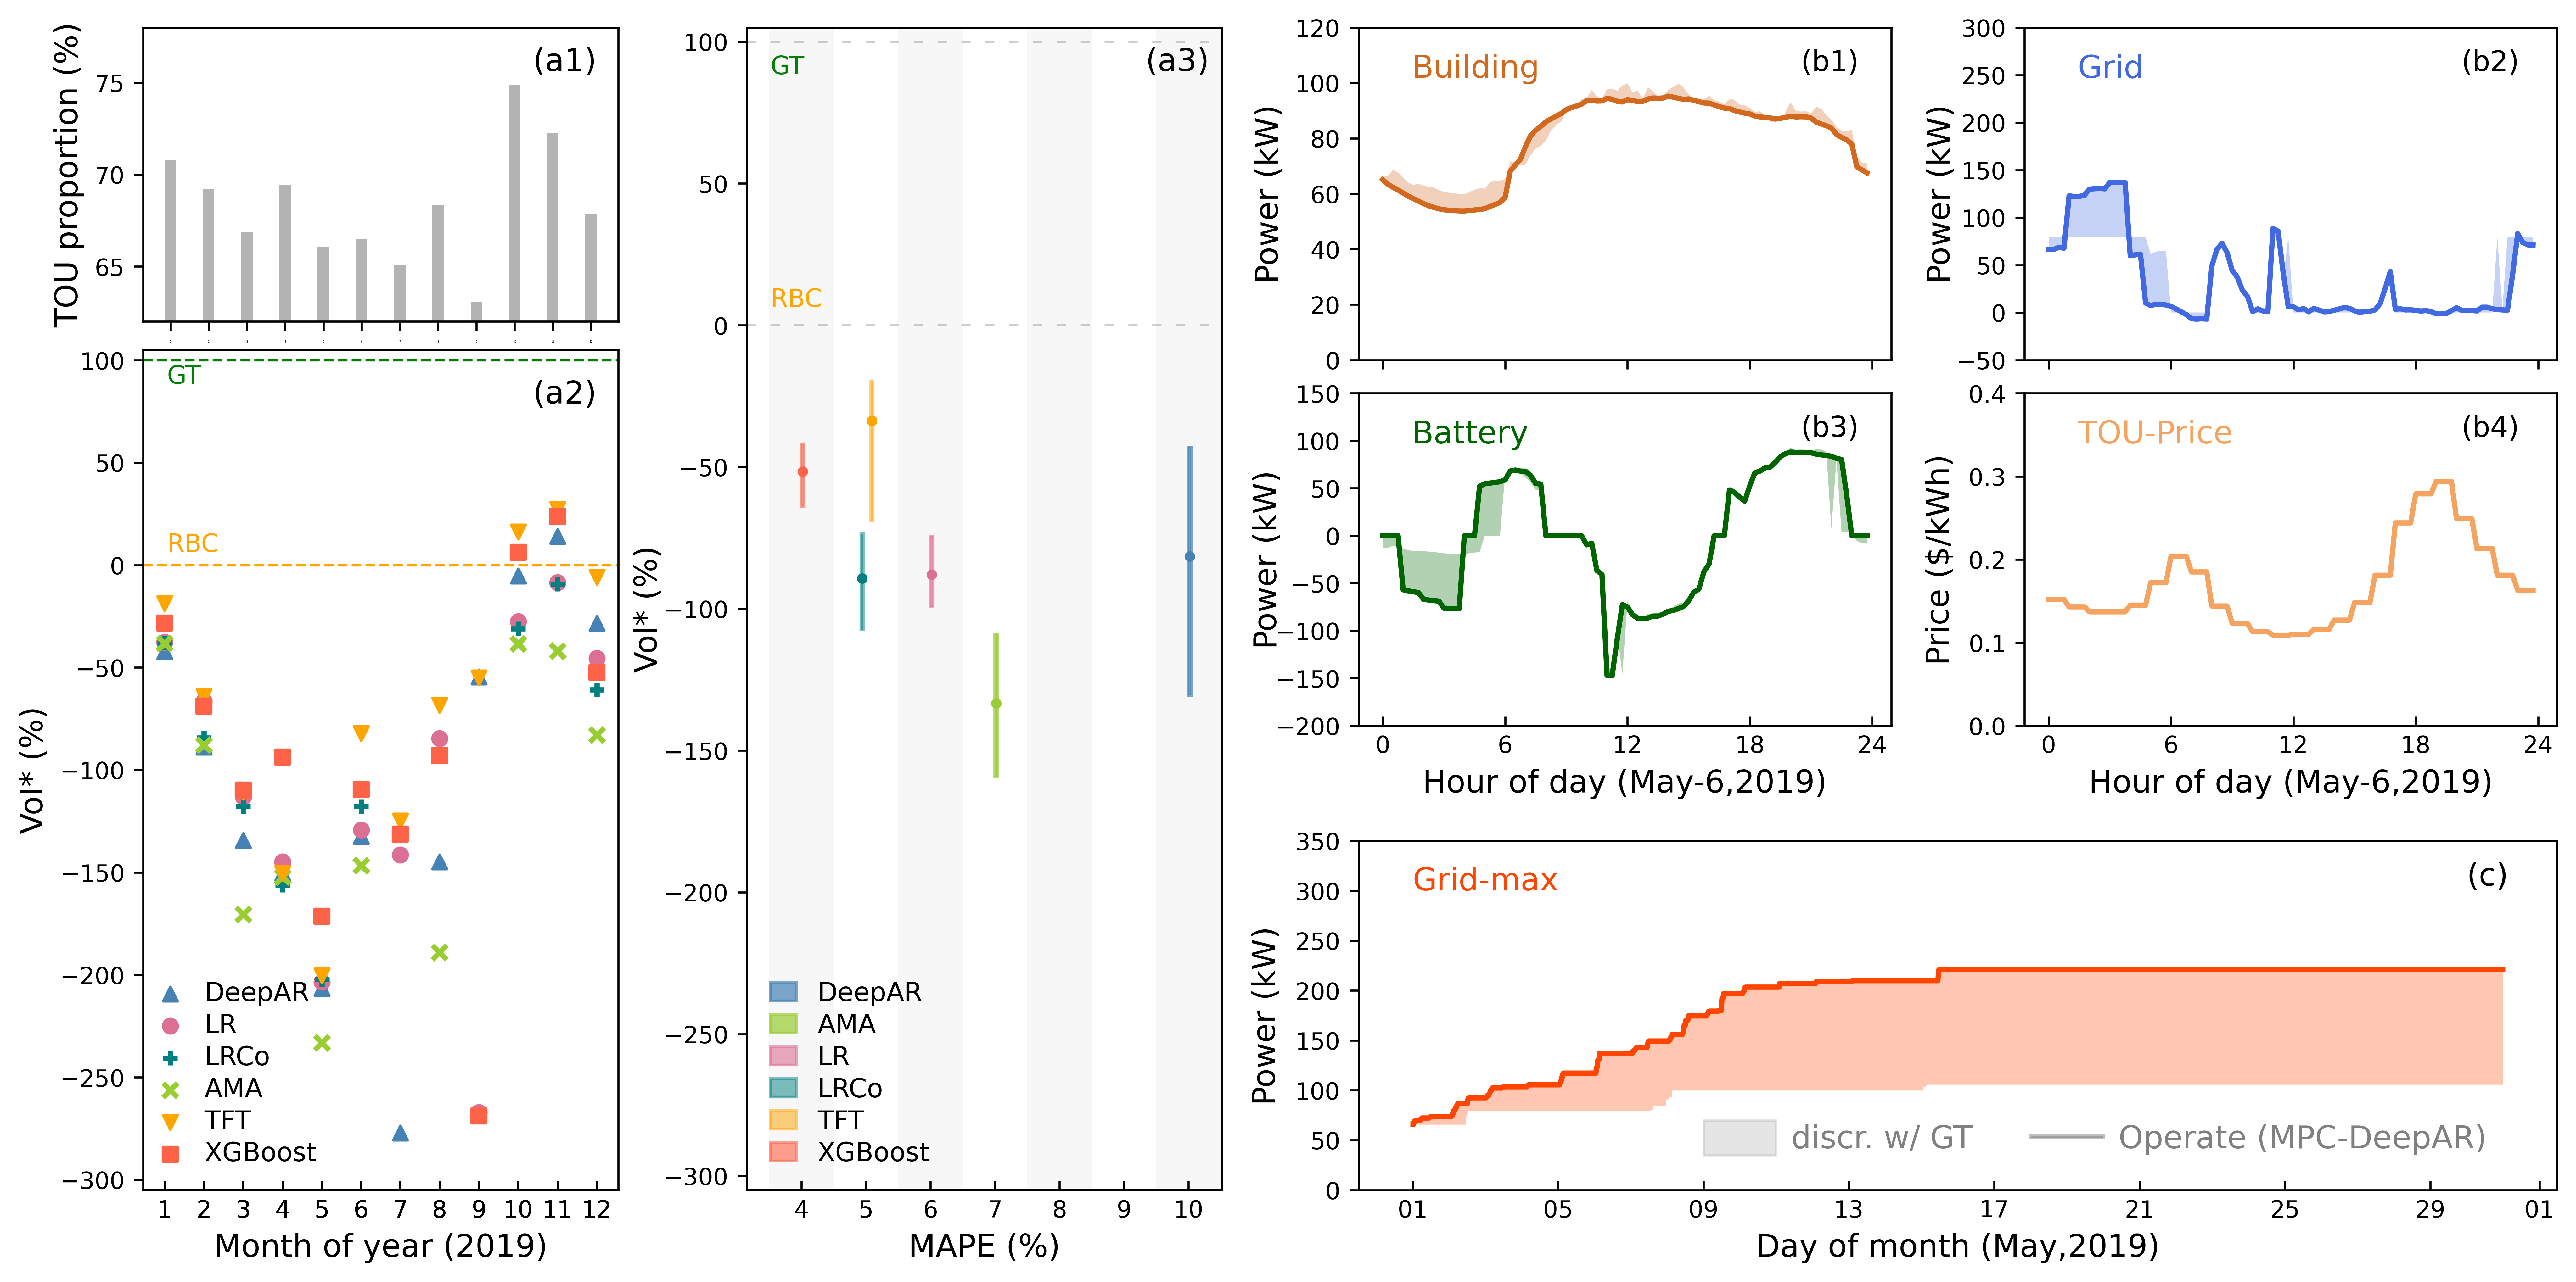
\includegraphics[width=1\textwidth]{figures/fig-3-with-dc-3.png}
  \caption{\textit{Control performance and sample control sequences under $\wdc$.} \textbf{(a1)} Bars show the proportion of TOU cost in the utility bill of month in year 2019. The values are calculated based on the \textbf{MPC-GT}. \textbf{(a2)} Each marker shows the performance of a monthly trial. Different marker styles represent prediction methods. $x$-axis shows months in year 2019 and $y$-axis is the corresponding normalized value of information (VoI*). \textbf{(a3), (b1)-(b4) and (c)} follow the same rules as in Fig. \ref{fig:group-plot-0dc}.}
  \label{fig:group-plot-dc}
\end{figure}


%As demand charge is taking a considerably-large proportion of electricity bills, particularly for the commercial and industrial sectors, it is crucial to consider it in  microgrid-related research. 
Under the scenario of $\wdc$, we applied a demand charge rate of 18\$/kW per month while maintaining other configurations unchanged. The corresponding results are presented in Fig.\ref{fig:group-plot-dc}. The control performance is significantly worse than under $\wodc$. And even the MPC with the best forecasts, XGBoost in this study, has inferior control performance in comparison to the baseline RBC. 

Based on the sample control sequences shown in Fig. \ref{fig:group-plot-dc}-\textbf{b1} to \textbf{b4}, the majority of control actions show similarities to optimal ones, but fail in establishing the proper boundary of peak demand. In the initial 6 hours of the day, excessive power than needed was imported from the external grid to pre-charge the battery. These operations can yield benefits by storing energy for high-TOU-tariff hours. However, raising peak demand unnecessarily leads to a serious decline in economic performance. Throughout the billing cycle, the peak demand was pushed up successively up to 221.3 kW, which is much higher than the optimal level of 105.6 kW. 
Since demand charge makes up a significant proportion (around 25\% to 60\%) of utility bills, the OPEX rises higher than that of RBC. As the proportion of demand charge increases (i.e. the proportion of TOU cost decreases), the control performance worsens, which is demonstrated in Fig. \ref{fig:group-plot-dc}-\textbf{a1} and \textbf{a2}.


\subsection{Asymmetric impact of forecast errors}
    \label{sec:Asymmetric impact}

\begin{figure}[!ht]
\centering
  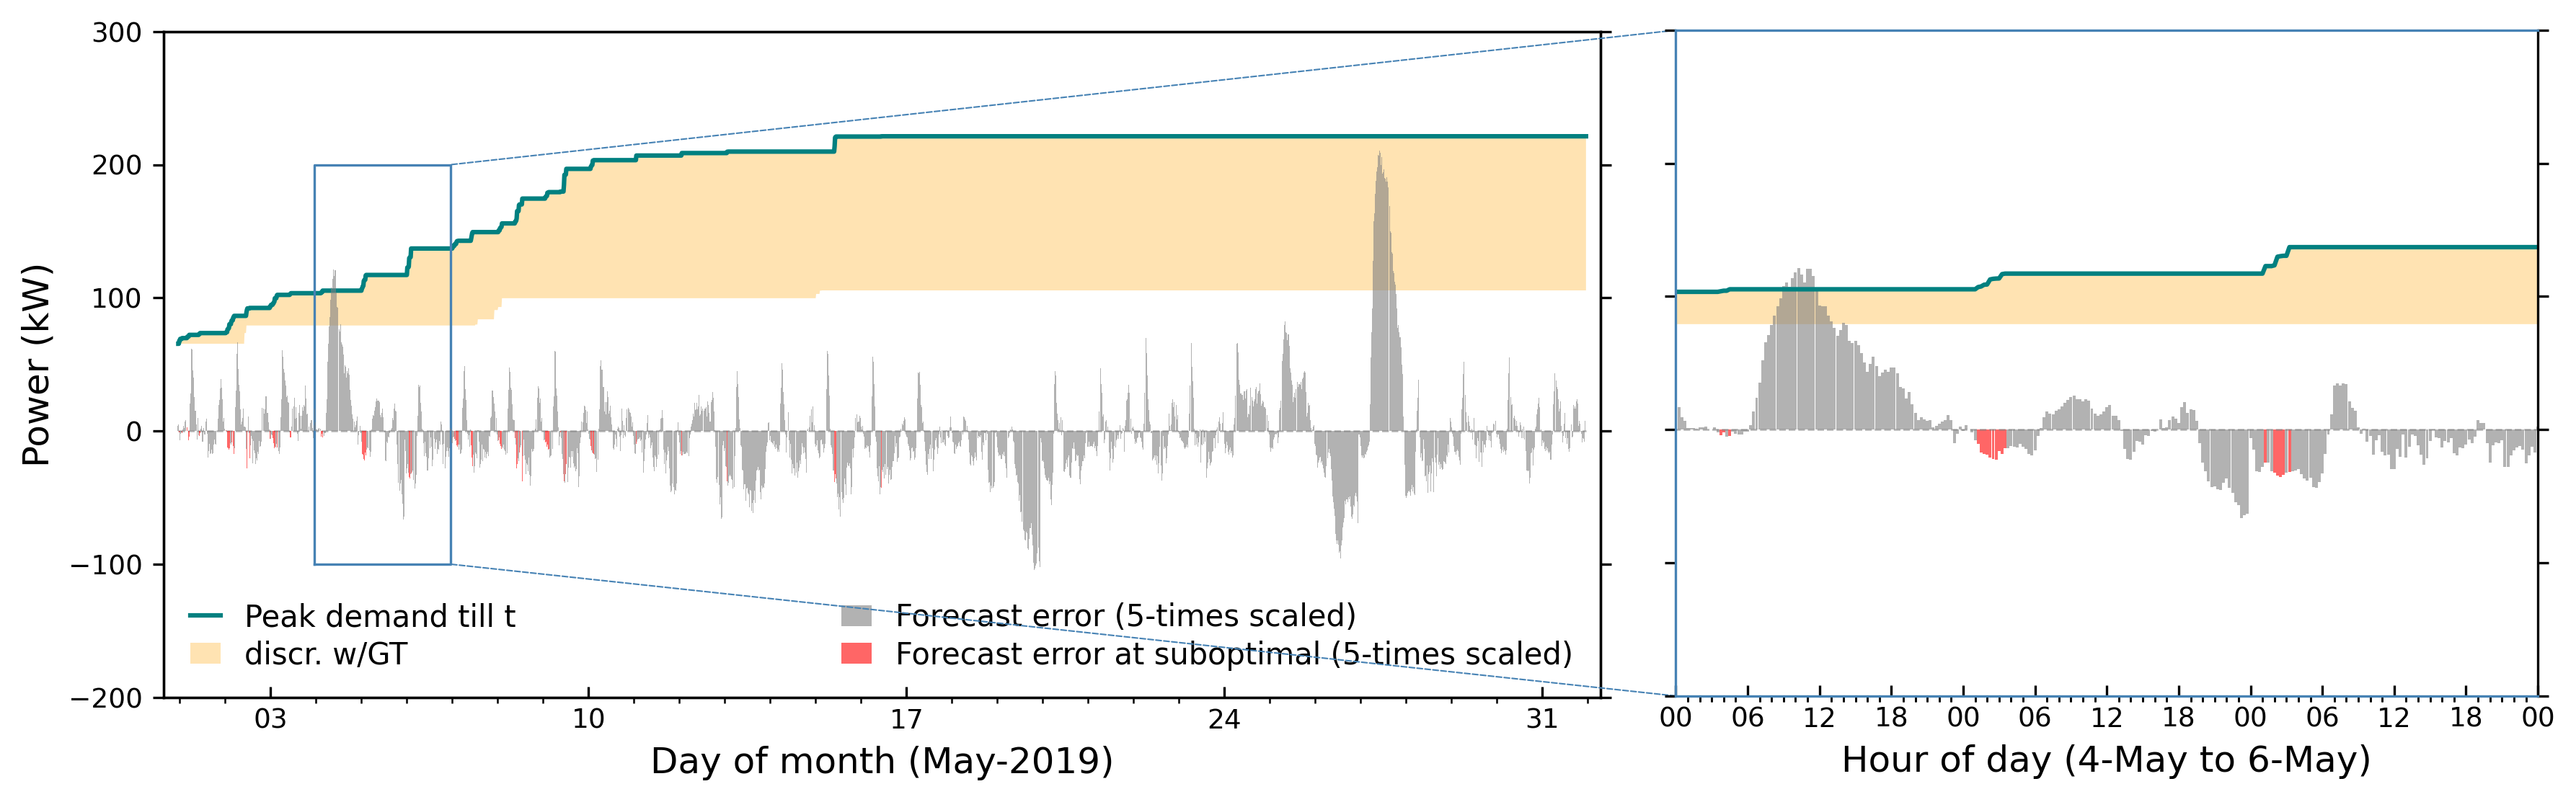
\includegraphics[width=1\textwidth]{figures/fig-9-track-peak-demand-and-error5.png}
  \caption{\textit{Track peak demand and forecast errors of \textbf{MPC-DeepAR} under $\wdc$}. Green line is the peak demand till time t of \textbf{MPC-DeepAR} control sequence. Yellow shaded area is the discrepancy of peak demand with MPC-GT. Gray bars are the forecast error at every time step. When the discrepancy (yellow shaded area) increases, the error bars are highlighted as red. All forecast errors are \textbf{5-times scaled up} for better visibility. }
  \label{fig:track-prak-demand}
\end{figure}


\begin{figure}[!ht]
\centering
  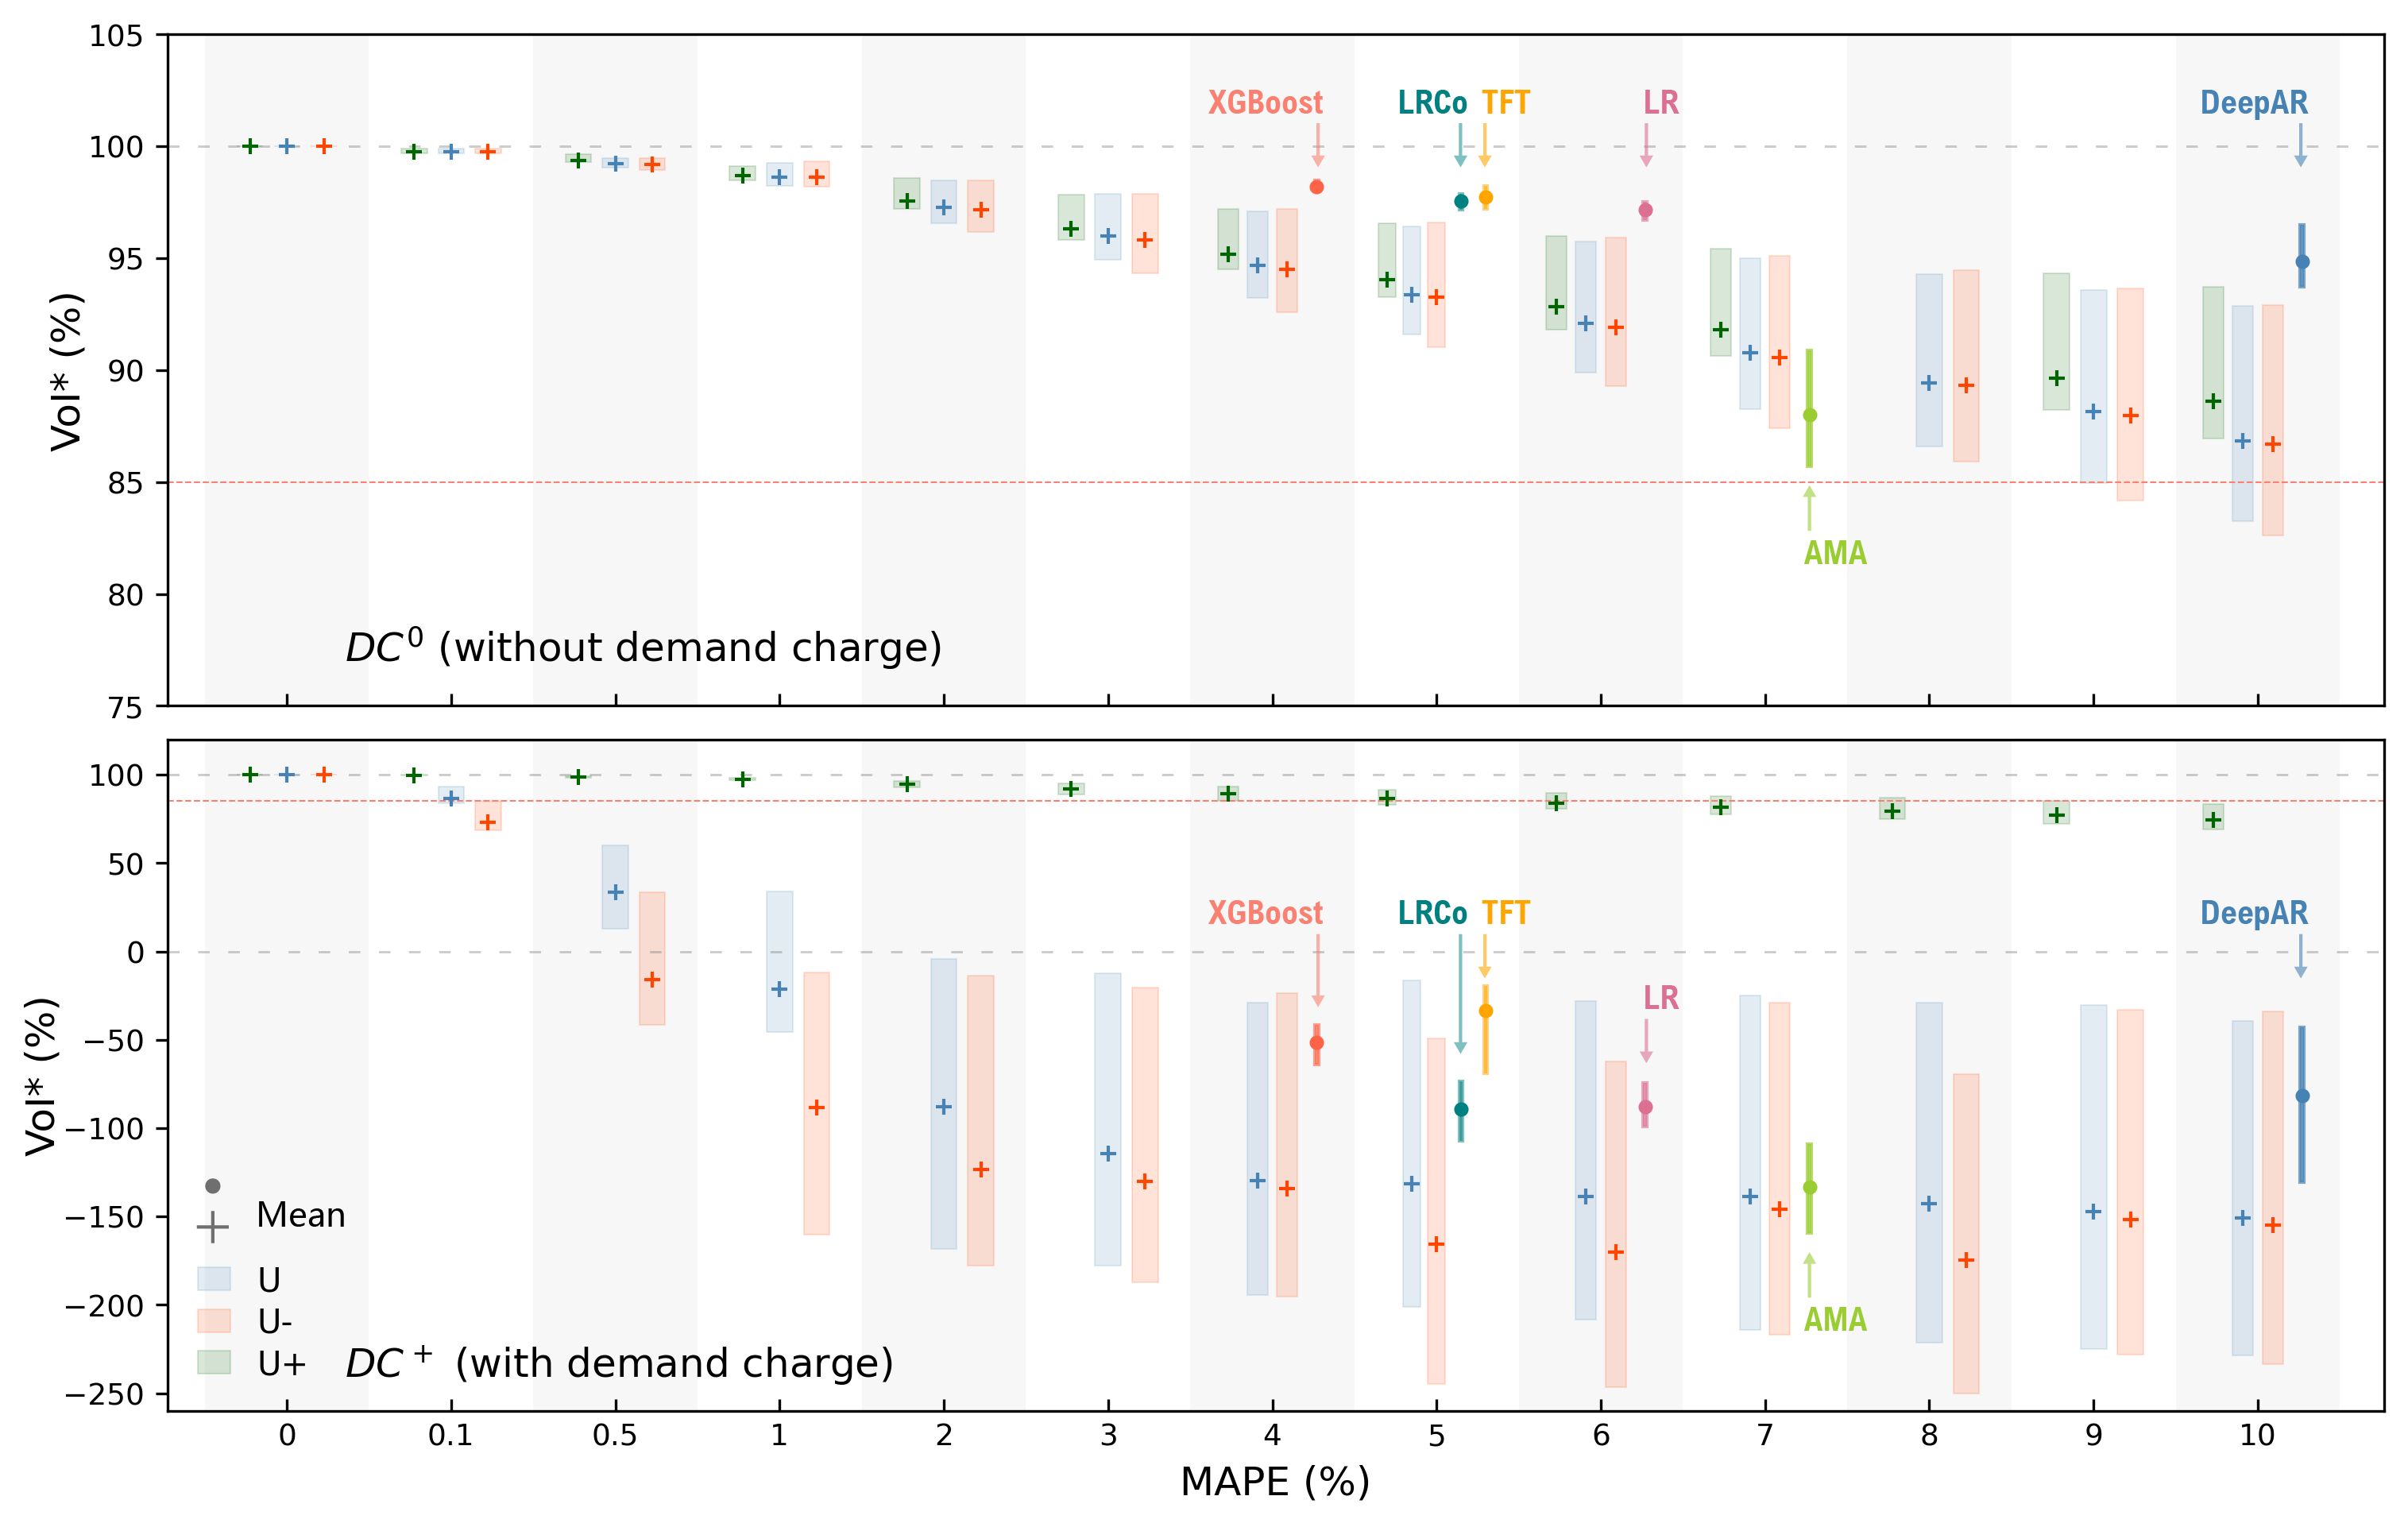
\includegraphics[width=0.85\textwidth]{figures/fig-4-VoI-artificial-noise-and-sota-models-combined 2.png}
  \caption{\textit{Control performance of $\MPCe$ and \textbf{MPC-ML} under $\wdc$ and $\wodc$.} $x$-axis shows the magnitude of forecasts, and $y$-axis is the corresponding normalized value of information (VoI*). Semi-transparent bars are performances of $\MPCe$, colors represent noise directions (blue: unbiased, orange: underestimate, green: overestimate). Narrow bars with emphasized colors are performances of \textbf{MPC-ML}, as noted in the tags. Each bar marks the 25\% and 75\% percentiles of trials for 12 months in 2019. ``+" and ``·" marks their mean values. Note the $x$-axis ticks are not even. Gaped gray shading areas merely help with identifying bars within one MAPE group.}
  \label{fig:VoI-group}
\end{figure}

When examining the trend of peak demand in conjunction with the forecast errors under $\wdc$, as depicted in Fig. \ref{fig:track-prak-demand}, it becomes evident that the forecast error exerts a biased influence. The tracked peak demand remains consistent with the optimal curve under load overestimates (up to 40 kW, i.e., 54.3\% of the yearly average load). It only deviates from and excesses the optimal one at time steps when the load is underestimated (marked as red bars). The explanation for this is that if the load is underestimated, more power needs to be imported from the external grid to maintain energy balance. This results in a higher executed $\pgrid_t$ than expected in the CFTOC solutions, consequently pushing up the tracked peak demand $\prevmax_t$ irreversibly. 

To further reveal the asymmetric impact of the forecast errors by decoupling it with the error magnitude, we generate synthesized forecasts by artificially adding random noises on true values. We consider adding three types of \emph{uniformly distributed} noises: for a given MAPE $\epsilon$, $\noise = \text{U}(-2\epsilon, 2\epsilon), \noisePos = \text{U}(0, 2\epsilon), \noiseNeg = \text{U}(-2\epsilon, 0)$, and forecasts
\begin{equation}
    \bldest_{t+k \mid t} = (1+\xi_{t+k}) \pbld_{t+k},\, \xi_{t+k} \sim \noise (\text{or }\noisePos, \noiseNeg) \,i.i.d. 
\end{equation}
%\yi{verbally explain this. - which is underestimates? which is overestimates? ...}
According to corresponding noises sampling rules, $\noisePos$ always overestimates the load whereas $\noiseNeg$ always underestimates the load, and $\noise$ generates unbiased forecasts.
Hereafter, we call MPC control with artificial noise as \MPCe. Then we vary the magnitude of forecasting MAPE from 0.1\% to 10\%\footnote{This range is selected intentionally to cover the MAPE of all forecast methods used in previous sections from 3.80\% (XGBoost) to 9.83\% (DeepAR). The lower bound of 0.1\% aims at gapping forecast and ground truth.} for U, U+ and U-, and run the simulation month by month in 2019. Corresponding results are provided in Fig. \ref{fig:VoI-group}. We also mark the control performances with practical forecast models, i.e., ML and AMA models, on the same subplots in Fig. \ref{fig:VoI-group}.



%As shown in Fig. \ref{fig:VoI-group}, the biased impact of forecast error exists under both $\wodc$ and $\wdc$ but varies in its degree. (As depicted in the top subplot) Under $\wodc$, \MPCe with U+ marginally outperforms that with U and U-. Upon a 10\% MAPE, the disparity of VoI* between \MPCe with U+ and those with \hl{U-} or \hl{U} is roughly 2\%, which shows a subtle contrast. While \MPCe with U+ demonstrates notably superior performance to the other two options under $\wdc$, this is consistent with our previous explanation. 

Under $\wodc$, the control performances do not exert notable asymmetric impact. All tested cases have near-optimal performances, and corresponding average VoI* is higher than 85\%. However, for $\wdc$, the asymmetric impact of forecasting error is notable. $\MPCe$ with purely overestimating forecasts (\textbf{U+}) outperforms the others significantly, and it still has near-optimal performances. While MPC with other forecasts containing (more or less) underestimating errors has performance inferior to RBC for most cases. 
In general, the relationship between forecasting error (MAPE) and VoI* revealed by our simple $\MPCe$ model is consistent with other ``real" models (i.e. \textbf{MPC-ML} and \textbf{MPC-AMA}). Though these ``real" models generate nearly unbiased forecasts, their performance is slightly better than $\MPCe$ with \textbf{U} which has unbiased forecasts as well. And it is noteworthy that their variances across different months are significantly smaller. Moreover, VoI* is not monotonically increasing with the decrease of MAPE. For instance, \textbf{MPC-XGBoost} has lower MAPE than \textbf{MPC-TFT}, but its VoI* is not higher than that of \textbf{MPC-TFT} under $\wdc$. Such nuances hint us that more metrics besides MAPE need to be considered to characterizing the relationship between VoI* and load forecast accuracy. And we extend this part in the discussions. 



%Notably, under $\wodc$, MPC-ML outperforms \MPCe in terms of both VoI* and robustness\footnote {MPC-ML have similar control performances for 12 months of the year 2019. In the plot, it is indicated by shorter bars compared with MPC under other forecasts.}.Within two groups, forecasting MAPE and VoI* display a linear correlation, while the slopeness is higher for \MPCe.  Under $\wdc$, such correlation still exists for \MPCe. For MPC-ML, however, MAPE alone does not indicate the control performance. For example, TFT and LR-PCo demonstrate remarkably similar MAPEs (5.19\% and 5.18\%, respectively). However, their corresponding average VoI* are vastly different: -33.7\% for TFT and -89.3\% for LR-PCo.

%\yi{I have concern on this paragraph: all words convey an idea: our findings are very noisy and random?! Do not simply describe (confusing) findings without explanation. I would write: The relationship revealed by our simple MPC-e model is in general consistent with the results from our ``real'' models. Though most prediction models make nearly unbiased forecasts, their performances are a little bit better than that under U, and their variances across different months are also notably smaller. Moreover, VoI* is not monotonically decreasing with MAPE. Such nuances hint us that more metrics besides MAPE need to be considered to characterizing the relationship between VoI* and load forecast accuracy. We extend this in the discussion section. - even this paragraph can be completely moved to discussion.}
%\lunlong{I am trying to rewrite this paragraph.}
  




\section{Discussion} \label{sec:discussion}
%\lunlong{Discussion not drafted yet}
\subsection{Forecast residuals and control performance}


\begin{figure}[!ht]
\centering
  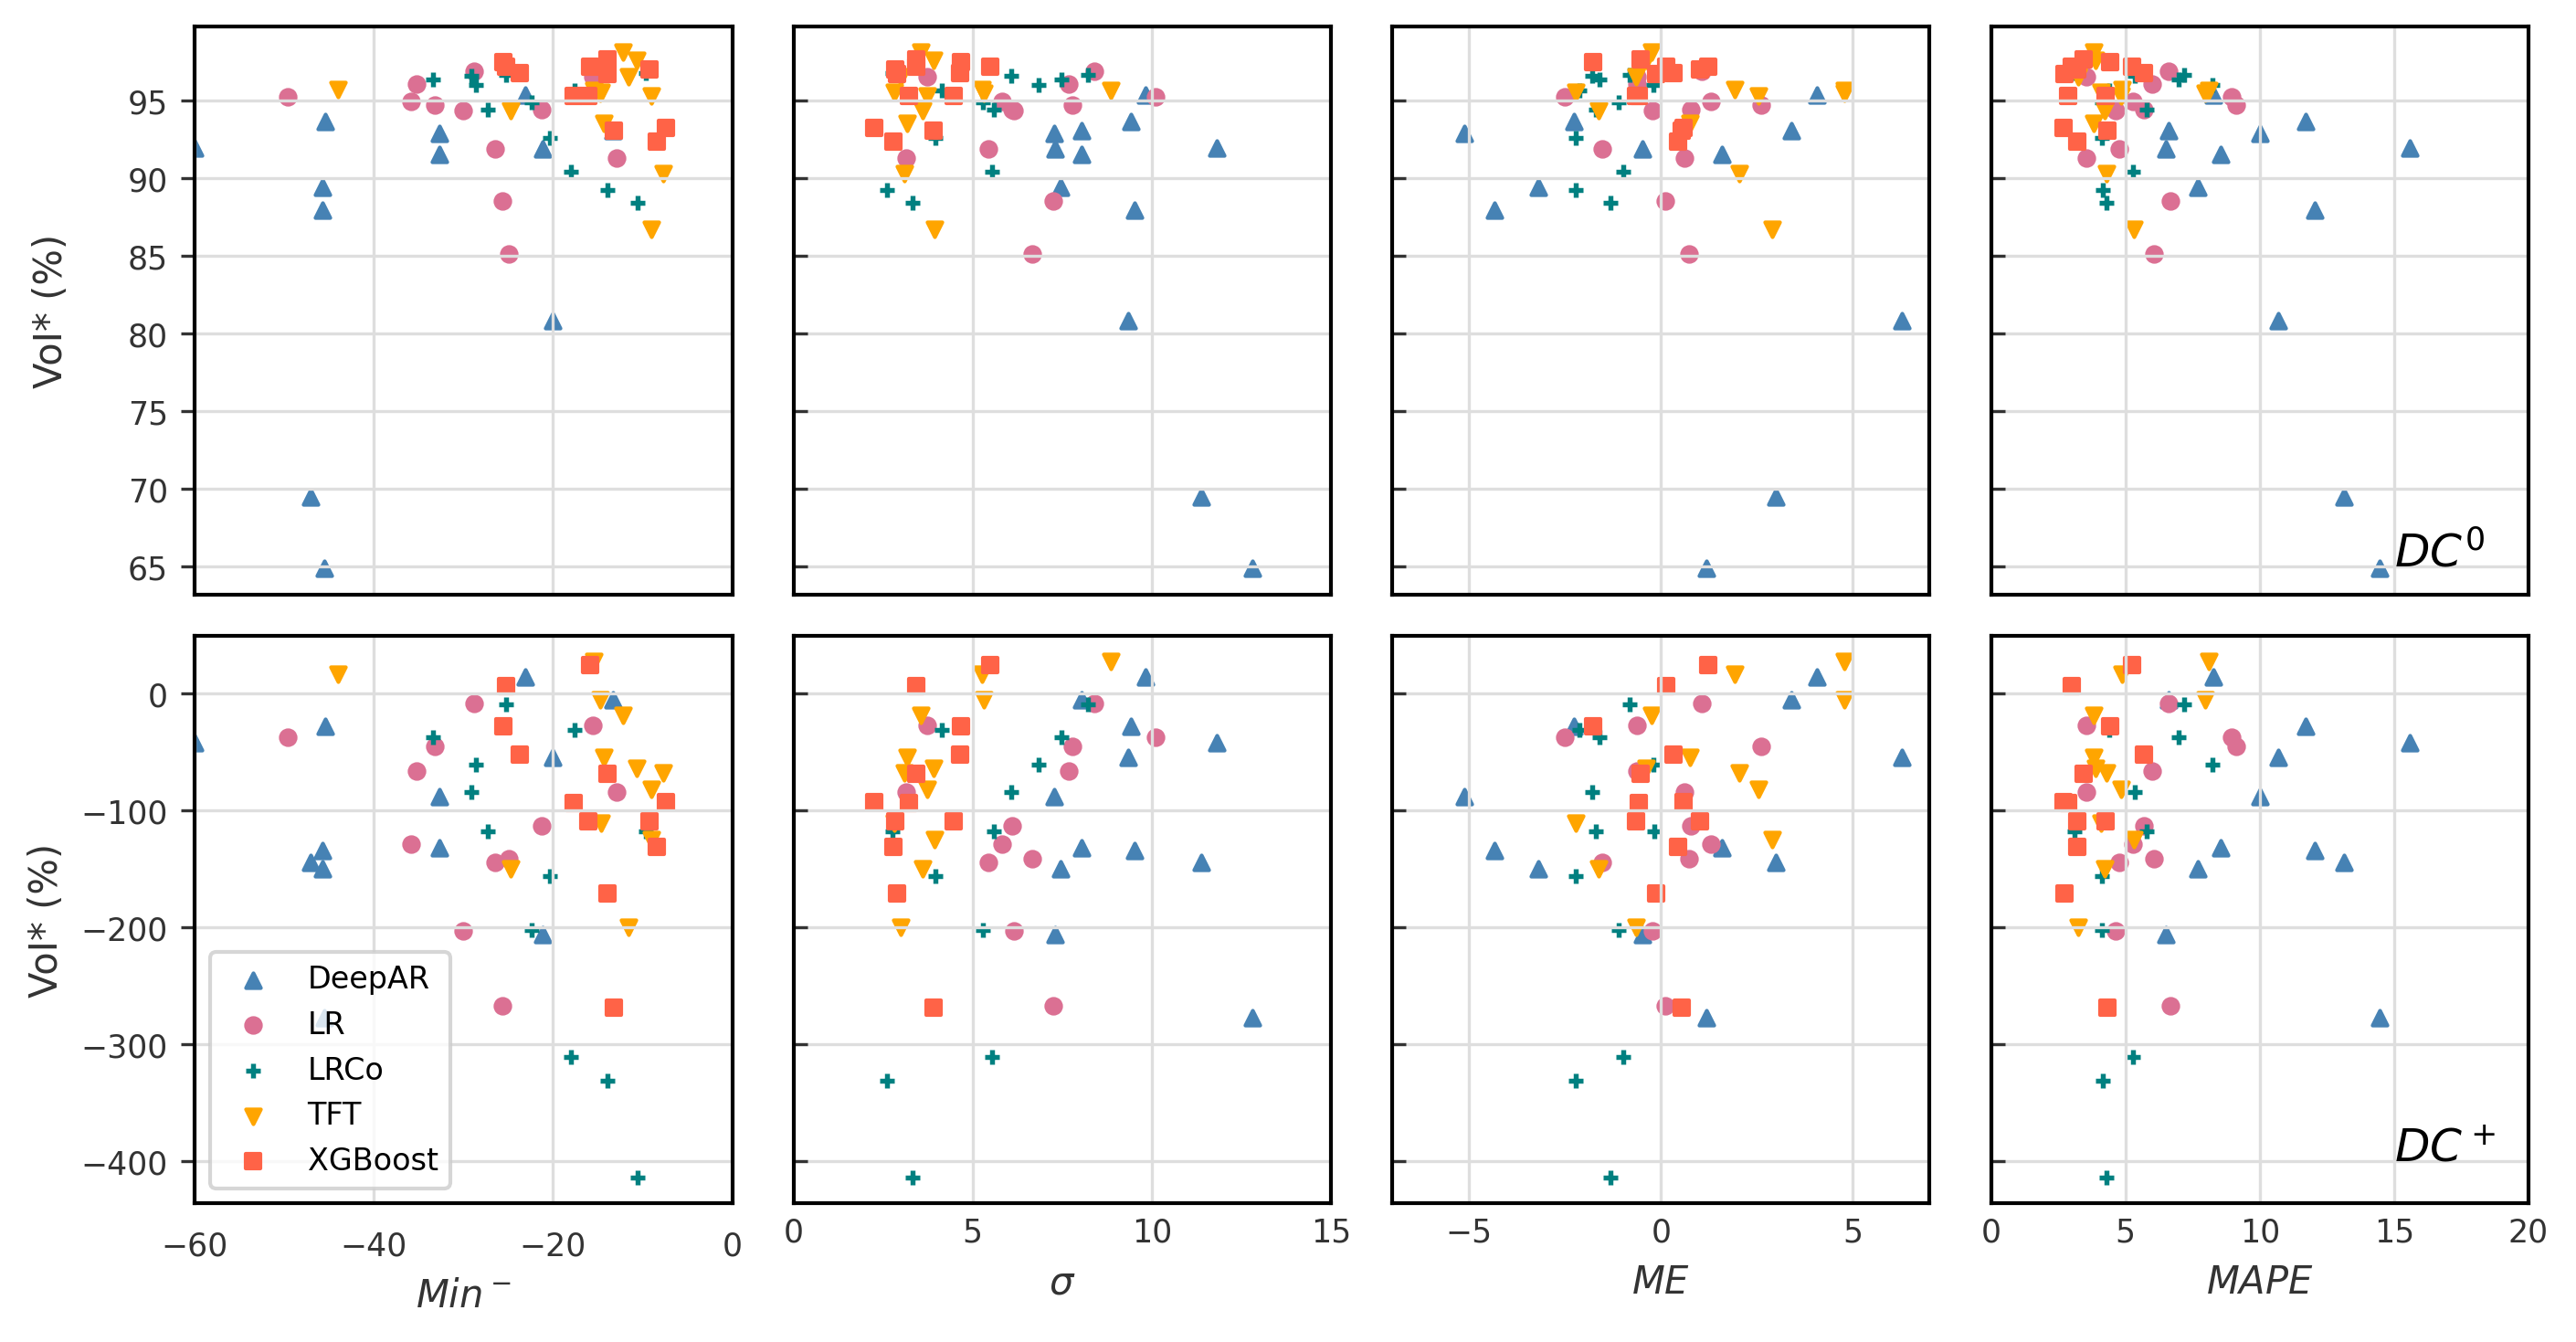
\includegraphics[width=1\textwidth]{figures/fig-10-VoI-metrics-pair-plot-2.png}
  \caption{\textit{} $x$-axis is values of metrics differed in each column. $y$-axis is the corresponding normalized value of information (VoI*). Each marker represents one monthly trial. Different forecast models are marked by varied markers. }
  \label{fig:VoI-metrics}
\end{figure}


\begin{figure}[!ht]
\centering
  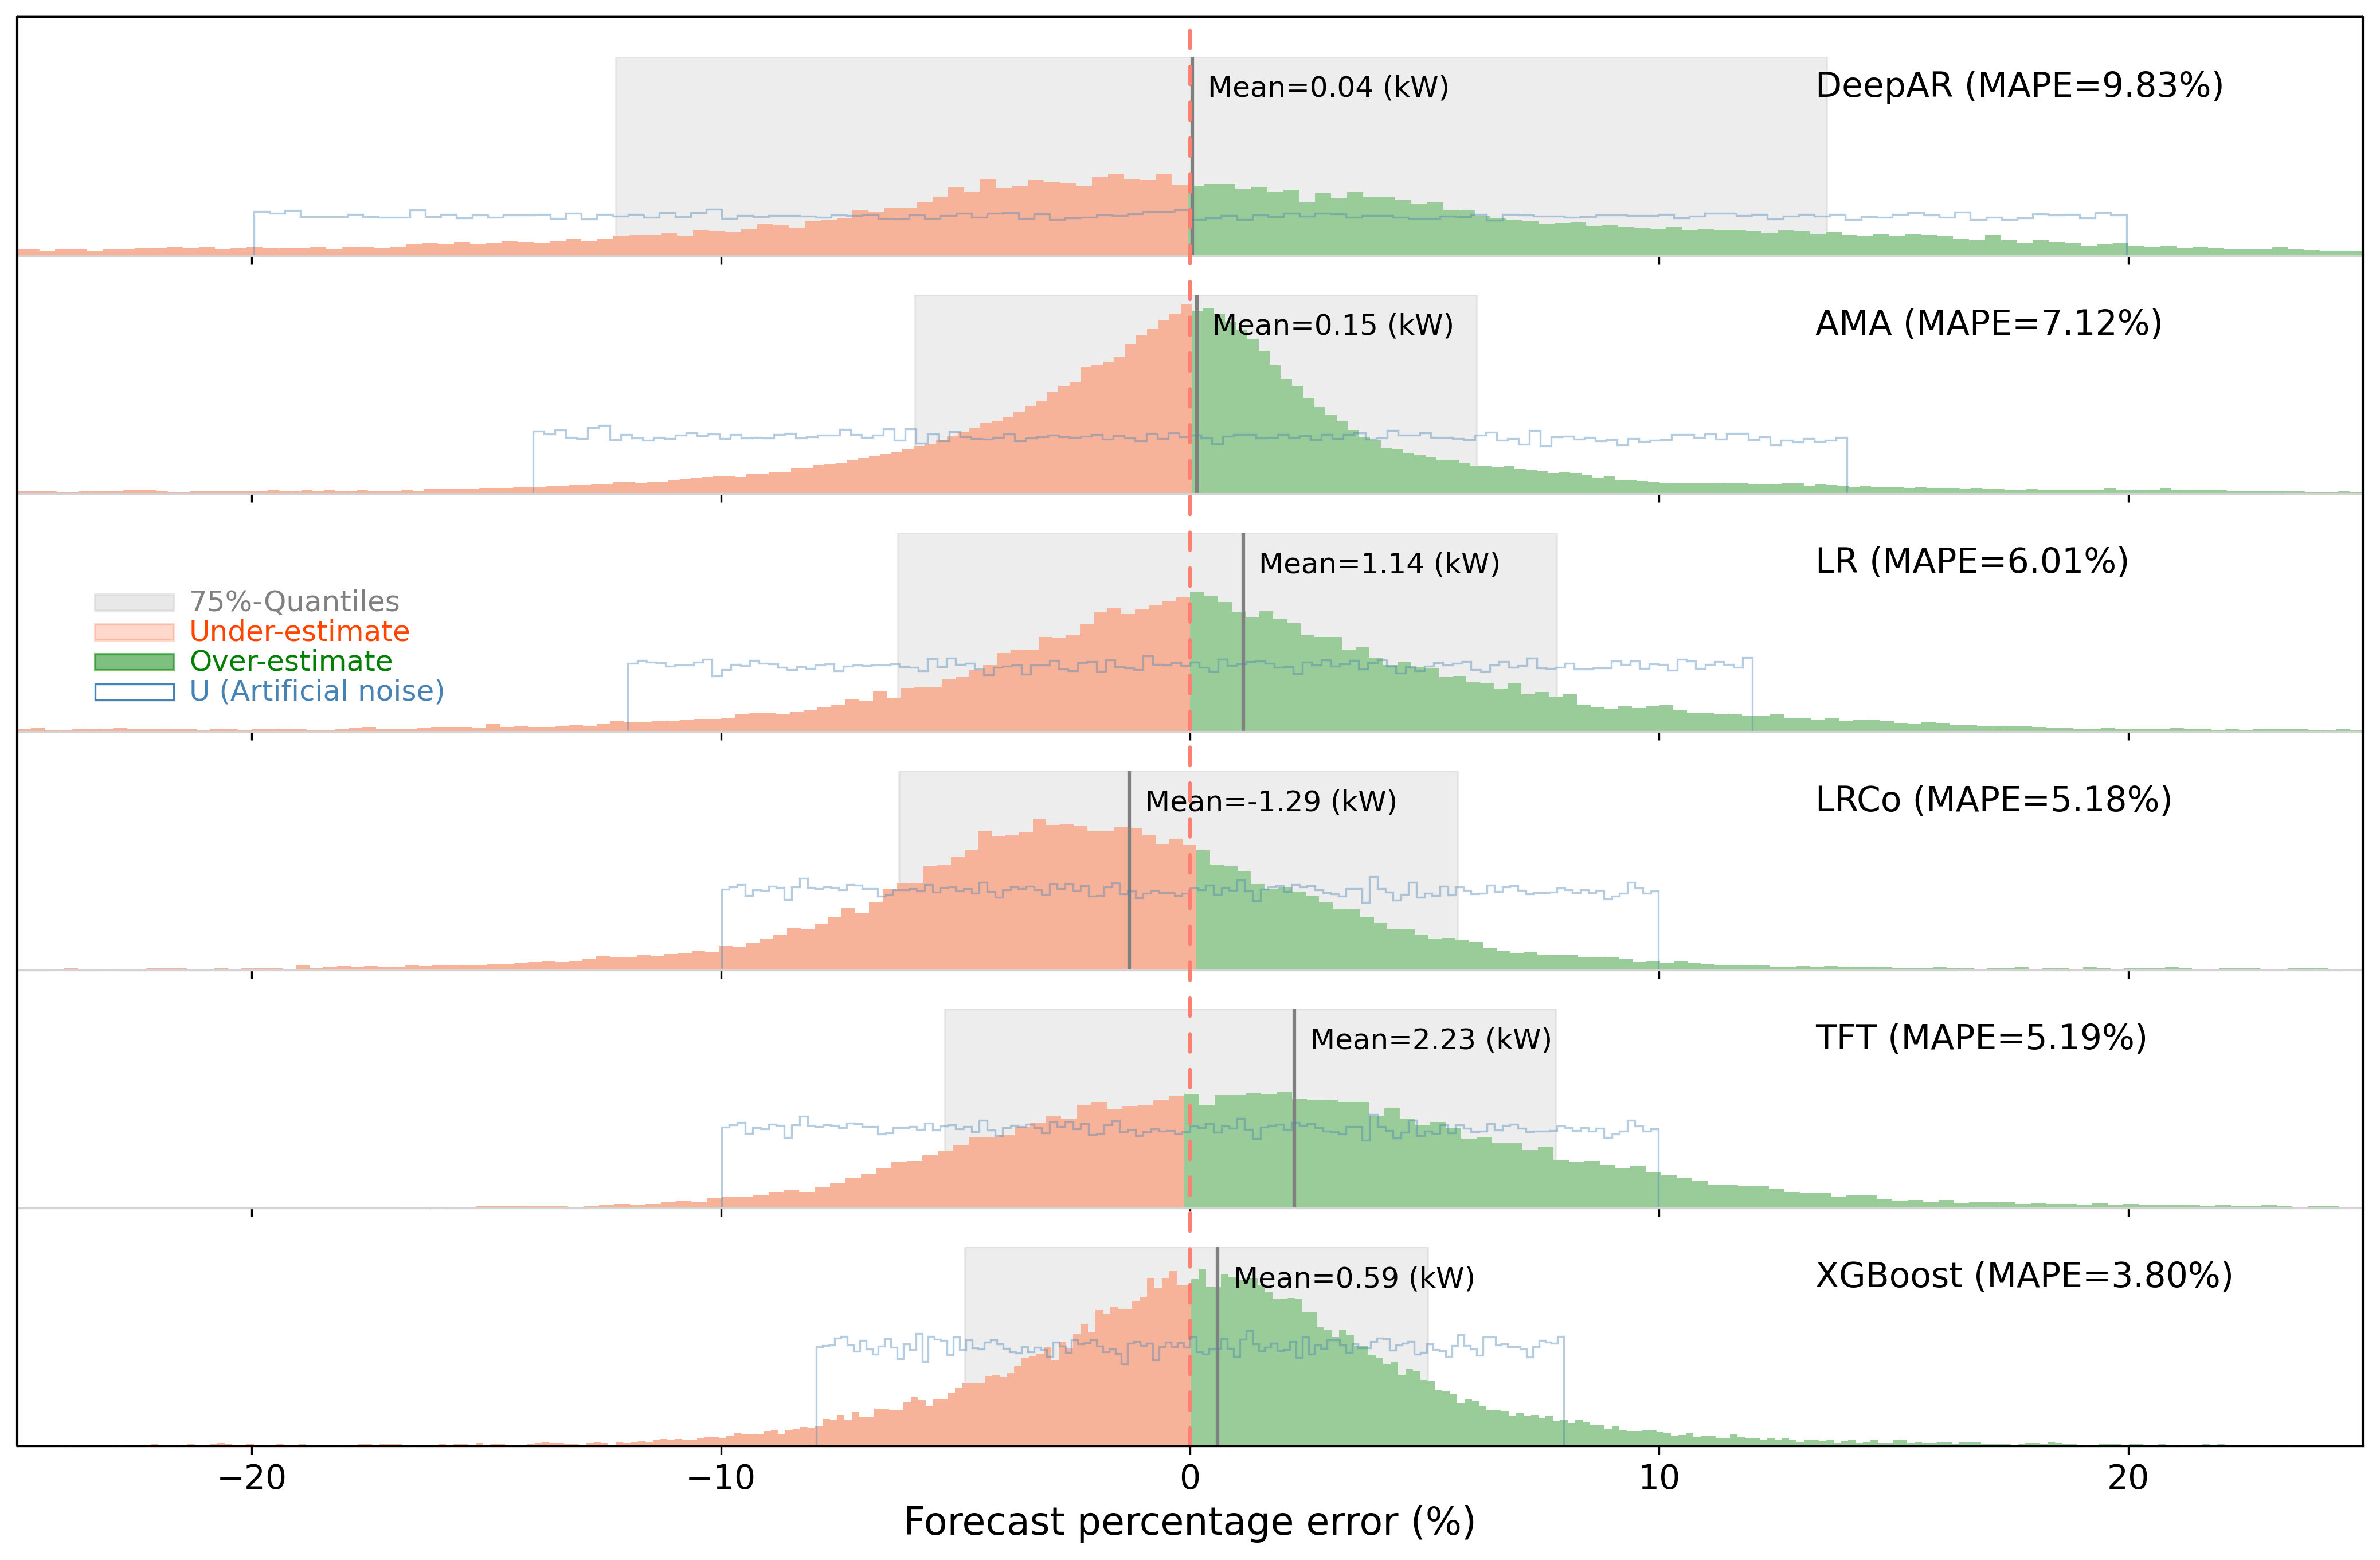
\includegraphics[width=0.85\textwidth]{figures/fig-7-residual-all.png}
  \caption{\textit{Forecast error distribution compared with artificial noise ($\textbf{U}$).} $x$-axis shows the value of forecast percentage error. Histogram in each subplot shows the error distribution of one specific prediction model tagged in the upper right. Orange bars are underestimated part, and green ones are overestimated part. Gray shading area marks the 75\% percentiles of the distribution. Mean value of forecasting errors is tagged. For comparison, the error distribution of unbiased artificial noise ($\textbf{U}$) is plot with blue lines, and corresponding magnitude, namely MAPE, is close to that of the model in the same subplot.}
  \label{fig:Error-distb-SOTA}
\end{figure}

The preceding observations suggest that the MAPE may not effectively serve as an adequate indicator of MPC's performance, especially when considering demand charges. Therefore, we incorporated three additional metrics that encapsulate aspects of the \emph{worst-case} scenario, \emph{variance}, and \emph{magnitude of mean values} for forecast residuals, as outlined in Eqs. (\ref{eq:Min-}) to (\ref{eq:ME}), where $\widehat{y_t}$ and $y_t$ represent the forecasted and actual values, respectively. The minimum value of underestimation:

\begin{equation} \label{eq:Min-}
    Min^- = min \{\widehat{y_{t}}-y_{t}|0<t<n \}
\end{equation}
The standard deviation $\sigma$ indicating the fluctuation of residuals:
\begin{equation} \label{eq:Std}
    \sigma=\sqrt{\frac{1}{n}{\sum_{k=1}^n (\widehat{y_t}-\bar{y})^2}}
\end{equation}
The average value of forecasting errors:
\begin{equation} \label{eq:ME}
    ME = \frac{1}{n} \sum_{t=1}^{n} (\widehat{y_{t}}-{y_{t})}
\end{equation}
%\begin{equation} \label{eq:MAE-}
%    ME^- = \frac{1}{n} \sum_{t=1}^{n} min\{0,{y_{t}-\widehat{y_{t}}}\}
%\end{equation}

In order to observe more samples, we present the monthly values individually, as depicted in Figure \ref{fig:VoI-metrics}. Notably, our chosen metrics exhibit a rather significant correlation with the VoI* metric under $\wodc$, with $\sigma$ and MAPE revealing a discernible relationship. However, under $\wdc$, increased uncertainties obscure such correlations, with only the ME metric indicating that higher ME values tend to correspond to higher VoI* outcomes.

Moreover, analyzing the distribution of forecast residuals may provide more insightful information for interpreting the influence of forecast errors, as shown in Fig. \ref{fig:Error-distb-SOTA}. It is evident that the forecast residuals distribute normally and have a more centralized distribution compared to artificial noise. 
%The superior control performance of MPC-ML over \MPCe may be attributed to such differences.
Additionally, there are variations in the distribution pattern among different forecasts. DeepAR , AMA and XGBoost exhibit relatively symmetrical distribution.
%though XGBoost indicates a more centralized distribution that corresponds with the MAPE.  
TFT and LR demonstrate a greater amount of residuals in the overestimated section, clarifying why \textbf{MPC-TFT} and \textbf{MPC-LR} exceed performance expectations. This is attributed to overestimated forecasts shown to perform better under $\wdc$, as analysed in Sec. \ref{sec:Asymmetric impact}. LRCo, in contrast, have more underestimated residuals, thus \textbf{MPC-LRCo} exhibits performance inferior to TFT which has similar MAPE. 


These observations highlight the need for the development of synthesized error metrics to more comprehensively uncover the intricate relationship between forecast residuals and MPC control performance within the domain of microgrid management. Singular and lump metrics, while informative, can capture only a single dimension of the residual characteristics. Other factors tied to time series patterns hold greater significance for MPC control challenges, as they exert a direct influence on the execution stage of MPC strategies. Our future research endeavors will be dedicated to further exploring and elucidating these relationships.

%In this section, it is concluded that both centralizing forecast residuals and overestimation are beneficial for MPC in terms of control performance. Centralizing the residuals takes the leading role under $\wodc$, whereas under $\wdc$, overestimation significantly improves control performance due to the biased impact of forecast error.

\subsection{Value of forecasts in the scope of time}

\begin{figure}[!ht]
\centering
  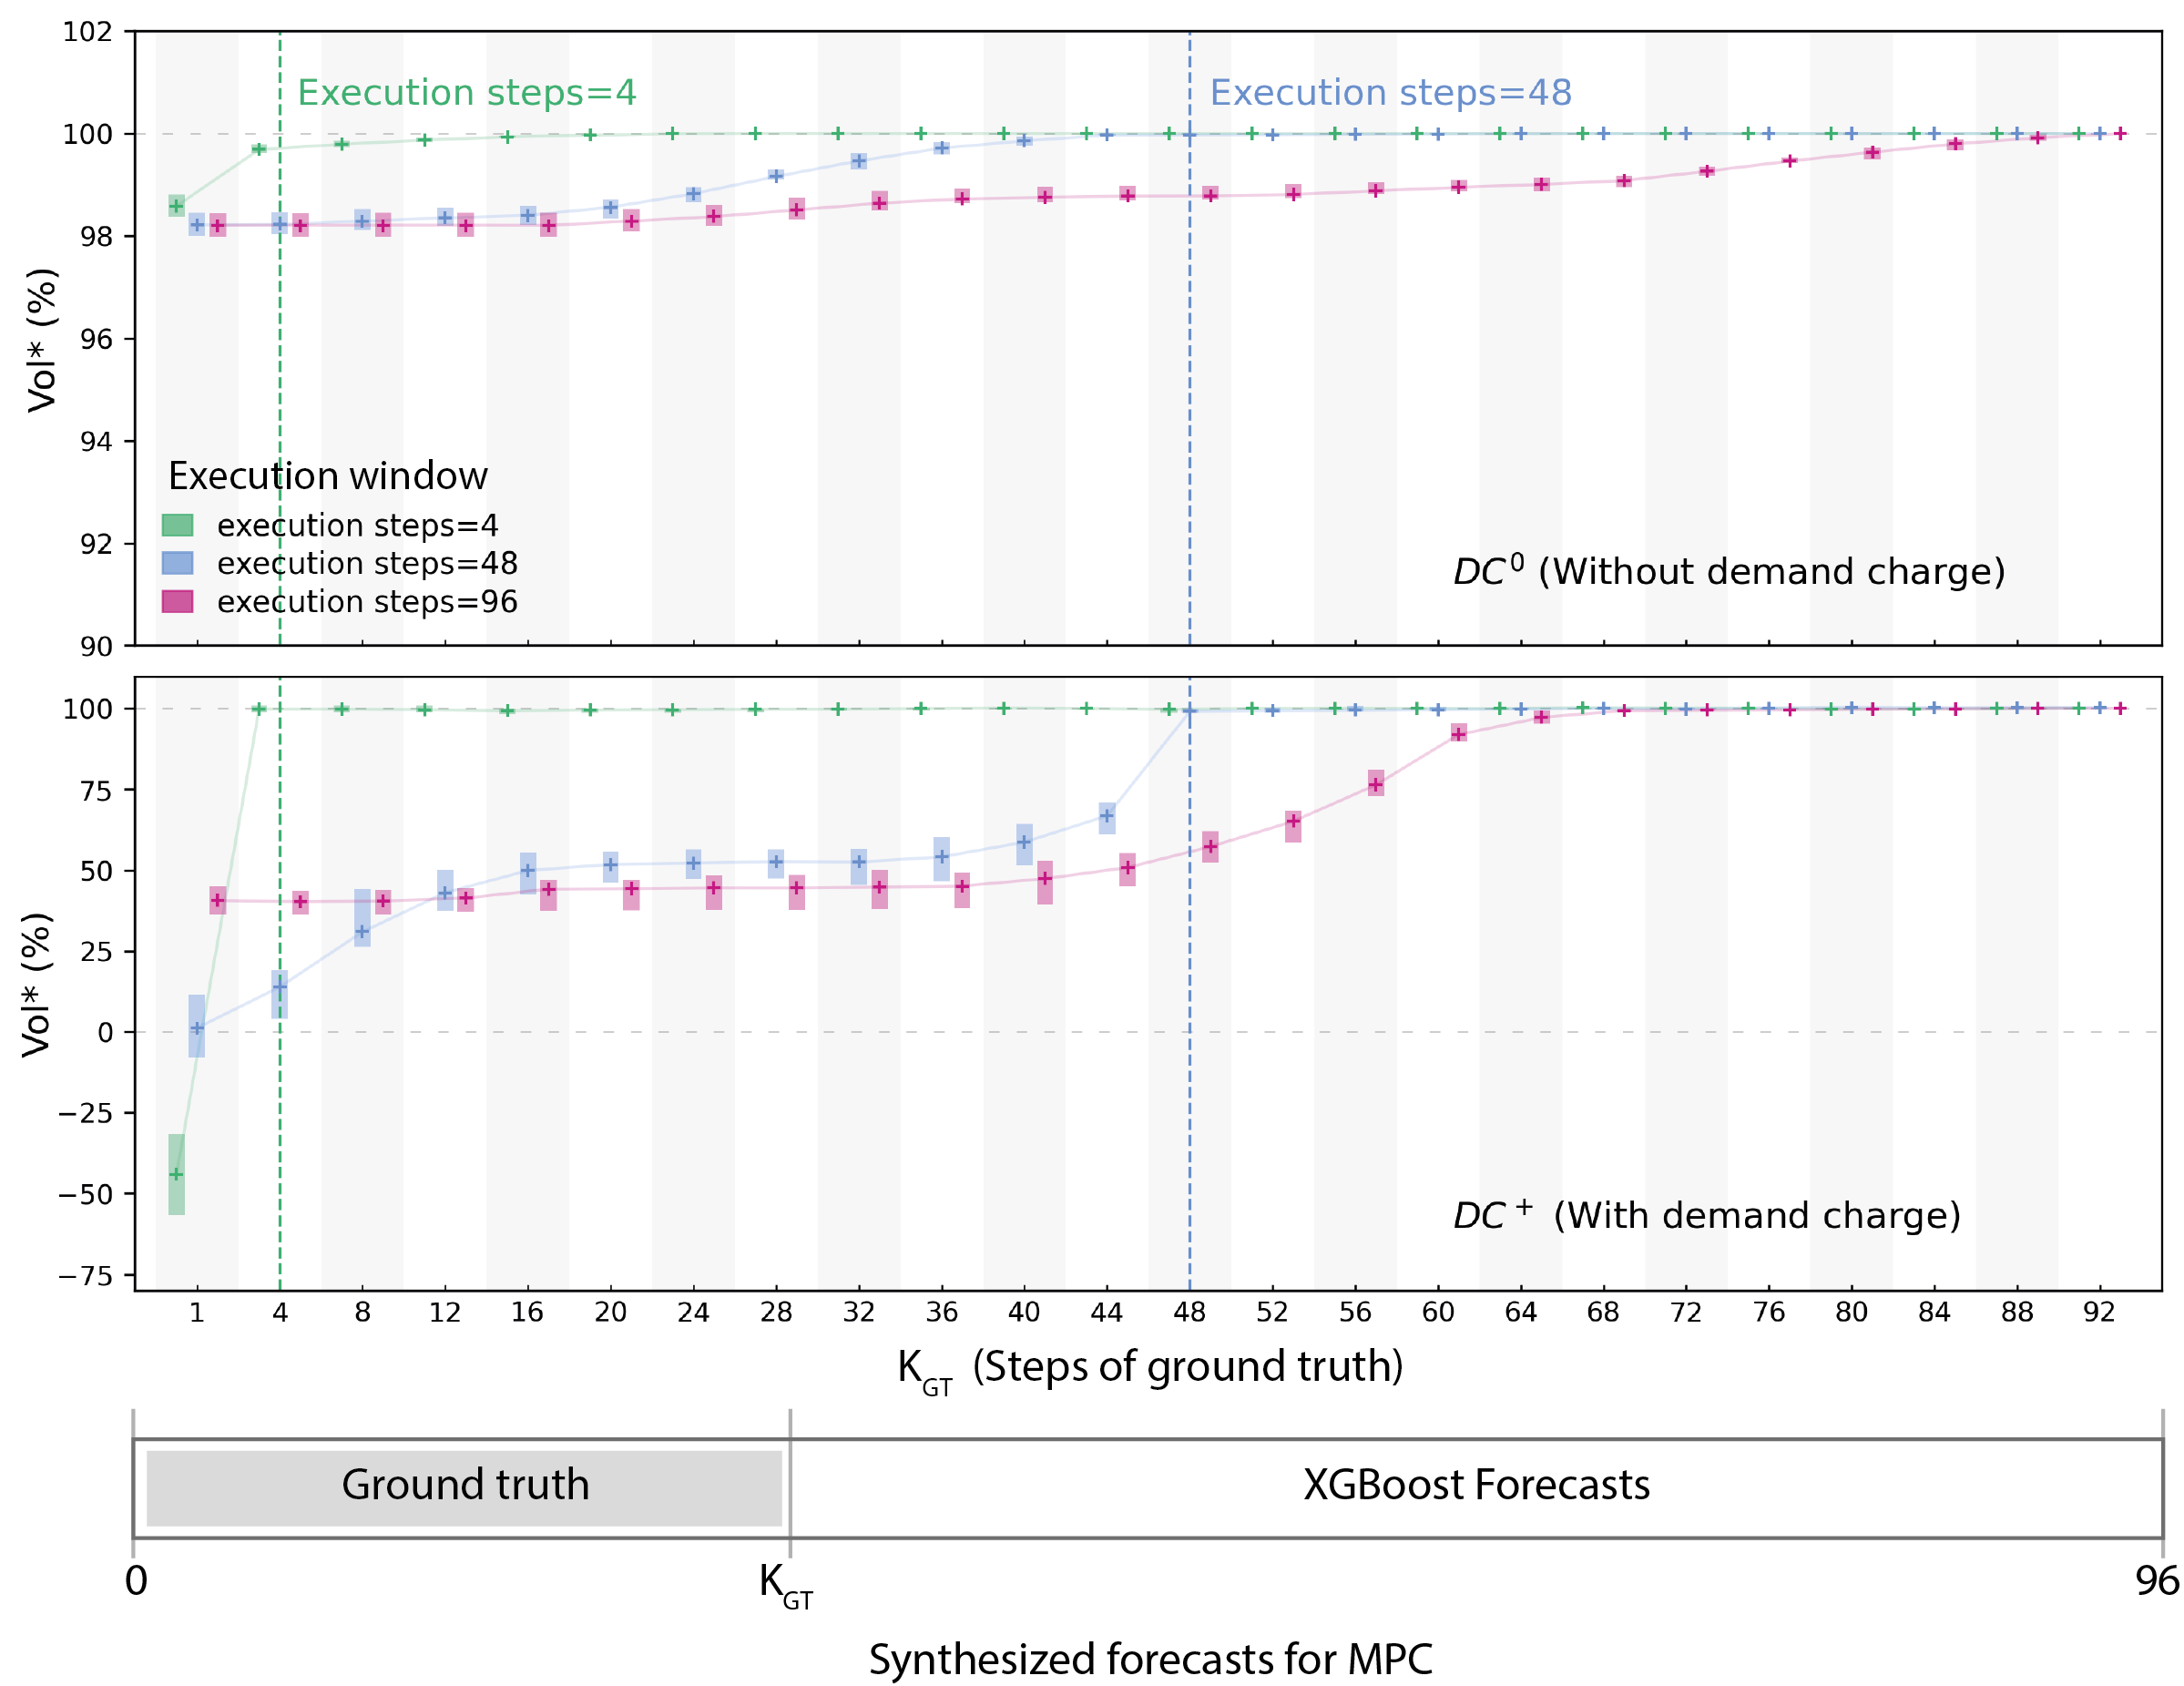
\includegraphics[width=0.85\textwidth]{figures/VoI_timescope.png}
  \caption{\textit{VoI* with varied forecast in time-scope.} $x$-axis is the steps of ground truth given to each CFTOC problem. How the forecasts are concatenated is shown in the diagram at the bottom. $y$-axis is the corresponding normalized value of information (VoI*). Each bar marks the 25\% and 75\% percentiles of trials for 12 months in 2019, and "+" marks their mean values. }
  \label{fig:VoI-timescale}
\end{figure}

In this study, the MPC optimization is a dynamic process. Within a single control window, K steps of forecasts are considered in the linear programming (LP), and only $\kexe$ steps of solutions are executed\footnote{In this study, K is set as 96 and $\kexe$ is 4, which correspond to 24h and 1h.}. Consequently, it is pertinent to examine the value of the prediction over time. A straightforward approach would be to create a combined prediction by merging accurate data with forecasts. As shown in Fig. \ref{fig:VoI-timescale}, we concatenate ground truth $\{\pbld_{t} \mid 0\leq t \leq \kgt\}$ and forecasts $\{\bldest_{t} \mid \kgt< t < K\}$ as synthesized forecasts for each step, and then conduct monthly simulations in 2019 while varying $\kgt$ between 0 and 96. The simulations were conducted in three groups for $\kexe$ values of 4, 48, and 96, as depicted by three colors.

The key observation is that the forecast error taking place within the execution window exerts a significant impact on control performance, compared to the negligible influence of errors occurring outside this window. This is because forecasts beyond the execution window help the LP detect and adapt to future trends, and associated errors do not have a direct effect on control performance. In contrast, forecast errors occurring within the execution window cause a direct mismatch between the solutions and executions, resulting in sub-optimality. 

Furthermore, there is another phenomenon that is somewhat counter-intuitive. In the case of $\wodc$, frequent re-optimization yields better performance as expected albeit with limited improvement. However, under $\wdc$, frequent re-optimization leads to deteriorating control performance. As depicted in Fig. \ref{fig:VoI-timescale}, when $\kgt$ is 1 and under $\wdc$, MPC with execution window of 96 steps (purple bars) outperform that with 4 steps (green bars). As examined in Sec. \ref{sec:Asymmetric impact}, frequent re-optimisation leads to offering inaccurate information more frequently. Therefore, decreasing the frequency of optimization when highly-accurate forecasts are unavailable under $\wdc$ refines performance control and diminishes the computational load.





\section{Conclusion and future work} \label{sec:conclusion}
%\lunlong{Conclusion not drafted yet}

In this research paper, we investigate the influence of forecast accuracy on the control performance in the context of smart grid operation. This is of utmost importance because the ultimate goal is to achieve effective control performance rather than merely accurate predictions. Furthermore, the presence of different pricing schemes adds complexity to optimizing control performance. Particularly, the pricing scheme that includes demand charges in the utility bill poses a significant obstacle. The longer billing cycle associated with demand charges compared to time-of-use costs makes it challenging to effectively control demand charges within a short optimization window for Model Predictive Control (MPC). Therefore, we thoroughly analyze the impact of prediction uncertainties with and without considering demand charges, and our findings reveal the following three key points:

\begin{enumerate}
    \item When demand charges are not taken into account, MPC achieves near-optimal performance even when the Mean Absolute Percentage Error (MAPE) of forecast reaches 10\%. Improving the accuracy of the forecasts has a limited contribution to enhancing control performance. Moreover, the simple Adaptive Moving Average (AMA) model proves to be an ideal forecasting model as it is computationally efficient, requires minimal historical data, and achieves satisfactory forecasting performance. However, when considering demand charges, even 1\% MAPE significantly deteriorates control performance to a level lower than Rule-Based Control (RBC).
    \item Through simulations involving artificial noise, including underestimation and overestimation, we uncover the asymmetric impact of forecasts when demand charges are considered. Underestimating future load leads to a substantial increase in peak demand, resulting in poor control performance.
    \item Singular lump metrics such as MAPE cannot serve as reliable indicators of MPC control performance, especially when demand charges are involved. These metrics overlook the residual distribution patterns and temporal correlations, which hold valuable information for MPC. Therefore, more intricate forecast features should be considered, aiming to provide a clear objective for upstream forecasting tasks.
\end{enumerate}

Based on these findings, it is important to acknowledge certain limitations in this study. The testbed formulated in this research is relatively simplistic, as it does not account for electric vehicles, despite the growing trend of incorporating charging stations in microgrid management. Additionally, we did not investigate the battery degradation in the Battery Energy Storage System (BESS). Furthermore, we only examined a few system configurations, which may limit the generalizability of our findings.

In addition to the MPC strategy implemented in this study, there are several solutions available to address prediction uncertainties, such as robust MPC and stochastic MPC. As a next step, we plan to evaluate their performance. Both robust MPC and stochastic MPC incorporate forecast uncertainty into the optimization stage, which may help mitigate the asymmetric impact of forecasting errors revealed in this study.
%Another concentration for the future work is to further explore a synthesized metric for evaluating the forecasts, 


\iffalse 
In this paper, we investigate the value of building load prediction on microgrid energy management control performance, with an emphasis on the role of demand charge term. The key challenge is to eliminate the cumulative impact of load forecast errors on the control performance of an entire billing cycle. Our proposed ``track-necessary'' approach is easy to implement in practice and demonstrate robustness under forecast errors. Meanwhile, our finding on the asymmetric value of information encourages researchers to consider the learning and optimization problems as a whole in future works. 
\fi

\section{Acknowledgement} \label{sec:acknowledgement}
This study was supported by the National Science Fund for Excellent Young Scholars (Grant number 52322813). This work was supported in part by the Project of Hetao Shenzhen-Hong Kong Science and Technology Innovation Cooperation Zone (HZQB-KCZYB-2020083).

\section{Declaration of generative AI and AI-assisted technologies in the writing process}

During the preparation of this work the authors used \emph{DeepL} in order to polish the language. After using this tool, the authors reviewed and edited the content as needed and take full responsibility for the content of the publication.
%\section{Appendix} \label{sec:appendix}
%\lunlong{Conclusion not drafted yet}
\input{content/88-appendix}

% \appendices
% \input{content/88-appendix}

 \bibliographystyle{IEEEtran}
 \bibliography{content/references}